\documentclass[english,11pt,3p,number,sort&compress]{elsarticle}
\usepackage[T1]{fontenc}
\usepackage[latin9]{inputenc}
\usepackage{geometry}
\geometry{verbose,tmargin=2cm,bmargin=2cm,lmargin=2cm,rmargin=2cm,headheight=2cm,headsep=2cm,footskip=1cm}

\usepackage{color}
\usepackage{array}
\usepackage{float}
\usepackage{algorithm2e}
\usepackage{amsmath}
\usepackage{amssymb}
\usepackage{stmaryrd}
\usepackage{bm}
\usepackage{graphicx}
\usepackage{lipsum}
\usepackage{nicematrix}
\usepackage[normalem]{ulem}

%%%%%%%%%%%%%%%%%%%%%%%%%%%%%% LyX specific LaTeX commands.
%% Because html converters don't know tabularnewline
\providecommand{\tabularnewline}{\\}

%%%%%%%%%%%%%%%%%%%%%%%%%%%%%% User specified LaTeX commands.
%\usepackage[latin1]{inputenc}

\usepackage{natbib}
\usepackage{dsfont}
\usepackage{comment}
\usepackage{ifthen}    
\usepackage{lscape}
\usepackage{multirow}
\usepackage{booktabs}
\usepackage{hyperref}

\usepackage[subpreambles=true]{standalone}
\usepackage{xspace}
\usepackage[percent]{overpic}

%tikz stuff
\usepackage[customcolors]{hf-tikz}
\usepackage{tikz}
\usepackage{pgfplots}
\usetikzlibrary{calc,shadings,patterns,tikzmark, plotmarks, spy, 
pgfplots.polar, external, matrix, shapes.symbols,shadings,shapes, 
decorations.shapes,decorations.pathmorphing,fit,backgrounds}
\pgfplotsset{compat=1.10}   %% <-- this added

\usepgfplotslibrary{groupplots}
\usetikzlibrary{calc}
\usepackage{pgfplotstable}

\usepackage{xcolor}

% WARNING: This folder must exist
\tikzexternalize[prefix=./figs_pgfplots/tikz/]

\newcommand{\includetikz}[1]{%
	\tikzsetnextfilename{#1}%
	\input{#1}%
}

% Commands for equations
\newcommand{\m}{\,\text{m}}

% compatibility for pgf figure
\pgfplotsset{compat=newest}

\hypersetup{urlcolor=blue, colorlinks=true}

% Useful when sending to journals.
% Do not provide path to figures in includegraphics comand. Set them
% here instead.
\graphicspath{ {./figs/} }

% path to tikz files. Do not use path in \includetikz command
\makeatletter
\def\input@path{{./figs_pgfplots/}{./figs/}}
\makeatother

\makeatletter
\@ifundefined{showcaptionsetup}{}{%
 \PassOptionsToPackage{caption=false}{subfig}}
\usepackage{subfig}
\makeatother

\usepackage{babel}

\newcommand{\giovane}{\color{red}{\bf\Large GA} \color{cyan} }
\newcommand{\nathan}{\color{red}{\bf\Large NS} \color{cyan} }
\newcommand{\phil}{\color{yellow}{\bf\Large PD} \color{cyan} }

\newcommand{\jump}[1]
{
	\llbracket #1 \rrbracket
}

\newcommand{\smallcirc}{\text{\tiny{$\circ$}}}

\newcommand{\logLogSlopeTriangle}[5]
{
    % #1. Relative offset in x direction.
    % #2. Width in x direction, so xA-xB.
    % #3. Relative offset in y direction.
    % #4. Slope d(y)/d(log10(x)).
    % #5. Plot options.

    \pgfplotsextra
    {
        \pgfkeysgetvalue{/pgfplots/xmin}{\xmin}
        \pgfkeysgetvalue{/pgfplots/xmax}{\xmax}
        \pgfkeysgetvalue{/pgfplots/ymin}{\ymin}
        \pgfkeysgetvalue{/pgfplots/ymax}{\ymax}

        % Calculate auxilliary quantities, in relative sense.
        \pgfmathsetmacro{\xArel}{#1}
        \pgfmathsetmacro{\yArel}{#3}
        \pgfmathsetmacro{\xBrel}{#1-#2}
        \pgfmathsetmacro{\yBrel}{\yArel}
        \pgfmathsetmacro{\xCrel}{\xArel}
        %\pgfmathsetmacro{\yCrel}{ln(\yC/exp(\ymin))/ln(exp(\ymax)/exp(\ymin))} % REPLACE THIS EXPRESSION WITH AN EXPRESSION INDEPENDENT OF \yC TO PREVENT THE 'DIMENSION TOO LARGE' ERROR.

        \pgfmathsetmacro{\lnxB}{\xmin*(1-(#1-#2))+\xmax*(#1-#2)} % in [xmin,xmax].
        \pgfmathsetmacro{\lnxA}{\xmin*(1-#1)+\xmax*#1} % in [xmin,xmax].
        \pgfmathsetmacro{\lnyA}{\ymin*(1-#3)+\ymax*#3} % in [ymin,ymax].
        \pgfmathsetmacro{\lnyC}{\lnyA+#4*(\lnxA-\lnxB)}
        \pgfmathsetmacro{\yCrel}{(\lnyC-\ymin)/(\ymax-\ymin)} % THE IMPROVED EXPRESSION WITHOUT 'DIMENSION TOO LARGE' ERROR.

        % Define coordinates for \draw. MIND THE 'rel axis cs' as opposed to the 'axis cs'.
        \coordinate (A) at (rel axis cs:\xArel,\yArel);
        \coordinate (B) at (rel axis cs:\xBrel,\yBrel);
        \coordinate (C) at (rel axis cs:\xCrel,\yCrel);

        % Draw slope triangle.
        \draw[#5]   (A)-- node[pos=0.5,anchor=north] {1}
                    (B)-- 
                    (C)-- node[pos=0.5,anchor=west] {#4}
                    cycle;
    }
}

\journal{Computer Methods in Applied Mechanics and Engineering}

\begin{document}

\begin{frontmatter}{}

%Um primeiro título
\title{A primal double-hybrid finite element method to solve tridimensional compressible, quasi-incompressible and incompressible elasticity using de Rham compatible H(div)-L2 spaces}

\author[uni]{Giovane Avancini}

\ead{giovanea@unicamp.br}

\author[uni]{Nathan Shauer}

\ead{shauer@unicamp.br}

\author[uni]{Hugo Luiz Oliveira}

\ead{hluiz@unicamp.br}

\author[uni]{Philippe R. B. Devloo}

\ead{phil@unicamp.br}

\address[uni]{Universidade Estadual de Campinas, R. Josiah Willard Gibbs 85 - Cidade Universitaria, Campinas SP, Brazil, CEP 13083-839}

%Definir se vamosar usar double-hybrid ou hybrid-hybrid. Adotei a segunda opção por enquanto
\begin{abstract}
	This work presents a novel primal double-hybrid finite element formulation for solving three-dimensional compressible, quasi-incompressible, and incompressible elasticity problems. Hybrid-mixed methods are typically derived from an extended variational principle, where interelement continuity requirements are relaxed and weakly enforced via Lagrange multipliers at element interfaces. In this context, we propose using a De Rham-compatible $H(\text{div})-L^2$ pair for displacements and pressure, respectively. The $H(\text{div})$ space naturally ensures normal displacement continuity across elements, while tangential continuity is recovered by introducing a shear stress approximation on element edges or faces, depending on the problem's dimension. This results in a semi-hybrid approach with two Lagrange multipliers, requiring the solution of a saddle-point problem even in the compressible regime. To overcome this drawback, hybridization is applied a second time to the shear stress which is statically condensed to recover a positive-definite block matrix that depends on the primal variable components. Although solving a saddle-point system remains necessary in the incompressible limit, numerical results demonstrate that this approach significantly enhances stability compared to the semi-hybrid formulation. Properties such as stability, consistency and local conservation are discussed in details. The formulation is tested and verified using 3D benchmarks for which analytical and/or numerical solutions are available, exhibiting optimal convergence rate, independent of the Poisson ratio. The proposed methodology is also applied to a real-world problem, where the robustness of the method is assessed.
\end{abstract}
\begin{keyword}
\textit{Mixed finite elements; Incompressible elasticity; $H\mathrm{(div)}$ approximation space; Hybridization}
\end{keyword}

\end{frontmatter}{}

\section{Introduction}

{\giovane A first shot, please give your contributions}
In the context of linear elasticity, several numerical methods have been developed in the past years. The most used one is the Finite Element Method (FEM). Using a continuous Galerkin approach to approximate the displacements may lead to shear-locking phenomenon due to spurious energy modes under bending \cite{bletzinger2000unified,belytschko1985stress} or volume-locking under quasi or full incompressibility, as the stresses go to infinity \cite{neto2005f,cervera2003mixed}.

There are different ways in the literature to overcome these drawbacks. One possible choice is to employ a mixed formulation \cite{brezzi2012mixed,arnold1988new} where the displacements and the stresses (or pressure) are approximated independently - i.e. the Taylor Hood elements \cite{taylor1973numerical} fulfill the \textit{inf-sup} condition yielding stable results for incompressible regime. This kind of approximation, on the other hand, is not locally conservative as it does not satisfy the divergence constraint in a strong manner. Another possibility is to use hybrid methods where the interelement continuity of a given field is broken and weakly imposed by means of a Lagrange multiplier (see for instance \cite{raviart1977primal,harder2016hybrid,farhloul1997dual}).

{\giovane escrevi esse texto na secao 5.1, mas ele fica melhor aqui.}In the context of Stokes-Brinkman flows, the authors in \cite{carvalho2024semi} developed a variant of the hybrid-mixed formulation that uses $H(\text{div},\Omega)$ velocity functions. In fact, the mixed problem of Eq. \eqref{eq:weak-mixed} and the hybrid version \eqref{eq:hybrid-weak} are stable, but none of them are locally conservative. This implies that, for Stokes flows, mass conservation does not hold strongly. Making a parallel to the incompressible elasticity, neither the incompressibility constraint is satisfied nor an equilibrated stress state is obtained element-wise.

In this work we extend the semi-hybrid approach proposed in \cite{carvalho2024semi} for Stokes flows to elasticity problems, developing a new formulation by performing a second hybridization on the tangential stresses. This formulation is based on a de Rham compatible pair $H(\text{div})-L^2$ for displacements and pressure. The $H(\text{div})$ functions are constructed using a systematic methodology described in \cite{devloo2022efficient,de2013new}.

\section{Preliminaries and notation}

Firstly, we introduce basic notation, functional spaces, and definitions that will be used throughout this work. Elasticity problems involve scalar, vector and tensor-valued fields. Hereinafter, vector fields are denoted by bold Latin letters, tensors are written using bold symbols or bold Greek letters, whilst plain Latin or Greek letters are chosen for scalars.

Let $\Omega \subset \mathbb{R}^d$, $d \in \{2, 3\}$, be a closed domain with Lipschitz boundary $\partial \Omega \subset \mathbb{R}^{d-1}$ whose  associated unit outward normal vector is denoted by $\bm{n}$. The scalar Hilbert spaces $L^2(\Omega)$ and $H^1(\Omega)$ have their usual meanings:
\begin{equation*}
    L^2(\Omega) = \left\{f: \int_{\Omega} f^2  ~d \Omega < \infty \right\},
\end{equation*}
\begin{equation*}
    H^1(\Omega) = \left\{v \in L^2(\Omega) : \partial_i v \in L^2 
    (\Omega) : i \in\{2,3\} \right\},
\end{equation*}

\noindent associated with their respective norms $\| \cdot \|_{L^2}$ and $\| \cdot \|_{H^1}$.

The space $H(\text{div},\Omega,\mathbb{R}^d)$ comprises square-integrable vector fields whose divergence is also square-integrable:
\begin{equation*}
	H(\text{div},\Omega,\mathbb{R}^d) = \left\{\bm{v} \in L^2(\Omega,\mathbb{R}^d) : \nabla \cdot \bm{v} \in L^2(\Omega) \right\},
\end{equation*}

\noindent equipped with the norm $\| \cdot \|_{H(\text{div})}$. {\giovane Henceforth, a space of vector valued functions is denoted by the symbol $\mathbb{R}^d, \,d \in \{2,3\}$. The same notation can be used for tensor fields, e.g. $\mathbb{R}^d \times \mathbb{R}^d$. Thus, \(L^2(\Omega,\mathbb{R}^d)=\{\bm{v} : v_i \in L^2(\Omega) : i \in\{2,3\} \}\).}

The notation used for the $L^2$ inner product is $(\cdot,\cdot)_{\Omega}$, while $\langle \cdot,\cdot\rangle_{\partial\Omega}$ stands for the duality pairing between the trace spaces
\begin{equation*}
	H^{1/2}(\partial\Omega,\mathbb{R}^d) = \left\{\bm{v}=\bm{u} \lvert_{\partial\Omega}, \bm{u} \in H^1(\Omega,\mathbb{R}^d)\right\},
\end{equation*}
\begin{equation*}
	H^{-1/2}(\partial\Omega,\mathbb{R}^d) = \left\{\bm{t}=\bm{\sigma} \,\bm{n} \lvert_{\partial\Omega}, \bm{\sigma} \in H(\text{div},\Omega,\mathbb{R}^d \times \mathbb{R}^d) \right\},
\end{equation*}

\noindent with $H(\text{div},\Omega,\mathbb{R}^d \times \mathbb{R}^d) = \left\{\bm{\sigma} \in L^2(\Omega,\mathbb{R}^{d \times d}) : \nabla \cdot \bm{\sigma} \in L^2(\Omega,\mathbb{R}^d) \right\}$ representing the space of tensor fields whose divergence is a vector field.

Let $\mathcal{T}_h=\left\{K_i \right\}, i\in \{1,...,N\}$ be a partition of $\Omega$ into non-overlapping elements $K$ with usual shape such that $\Omega = \cup_{i=1}^{N} K_i$. The boundary of each element is denoted by $\partial K$ with outward unit normal vector to the boundary $\bm{n}^K$. The set $\Gamma_h=\cup_{K \in \mathcal{T}_h} \partial K$ is named the mesh skeleton, and comprises the union of all element boundary segments (lines for 2D and facets for 3D). It can be decomposed into a boundary subset $\Gamma_{\partial\Omega}=\{E \in \Gamma_h : E \subset \partial\Omega\}$ and an interior subset $\mathring{\Gamma}_h =\{E \in \Gamma_h \setminus \Gamma_{\partial\Omega}\}$. Analogously, $\partial\mathcal{T}_h=\bigcup_{K \in \mathcal{T}_h} \partial K$ denotes the disjoint union of all element boundaries. Note that $\Gamma_h$ differs from $\partial\mathcal{T}_h$ since for every $E \in \mathring{\Gamma}$, the latter includes the boundaries from both adjacent elements.

Over an element interface $E \in \mathring{\Gamma}_h$ between two elements $K_i$ and $K_j$, the jump operator of a function $v$ is defined as
\begin{equation*}
	\jump{v}_E = v_i \lvert_{E} - v_j \lvert_{E} \text{.}
\end{equation*}

Moreover, a broken Sobolev space of the square-integrable functions on the discretized domain can be defined as
\begin{equation*}
	X(\mathcal{T}_h) = \left\{v \in L^2(\Omega) : v \lvert_{K} \in H^1(K), \,\forall \, K\in\mathcal{T}_h \right\} ,
\end{equation*}

\noindent and the space of functions whose trace normal component is continuous across elements is denoted by
\begin{equation*}
	\mathcal{V}(\mathcal{T}_h,\mathbb{R}^d) = X(\mathcal{T}_h,\mathbb{R}^d) \cap H(\text{div},\Omega) .
\end{equation*}

\noindent Both spaces $X(\mathcal{T}_h)$ and $\mathcal{V}(\mathcal{T}_h,\mathbb{R}^d)$ are equipped with the broken $H^1$-norm $\| \cdot \|_{H^1,\mathcal{T}_h}$ and the inner product $(\bm{u},\bm{v})_{H^1,\mathcal{T}_h}=(\bm{u},\bm{v})+\sum_{K \in \mathcal{T}_h}(\nabla\bm{u},\nabla\bm{v})_K$.

\section{Elasticity problem \label{sec:Governing-equations}}

In this section, the governing equations for the linear elasticity problem are defined. First, the primal displacement based formulation is presented, followed by the mixed version introducing the pressure as an indepent variable.

\subsection{Problem definition}

The conservation of linear momentum for a generic continuum body is given by:
\begin{equation} \label{eq:momentum}
		-\nabla \cdot \bm{\sigma} - \bm{b} = \bm{0} \hspace{0.2cm} \text{in } \Omega ,
\end{equation}
\noindent where $\bm{b}$ is the body force vector and $\bm{\sigma}$ denotes the Cauchy stress tensor. The Generalized Hooke's law relates the stresses and strains in a isotropic body as:
\begin{equation} \label{eq:hook}
    \bm{\sigma} = 2\mu \bm{\varepsilon}(\bm{u}) + \lambda \text{tr}(\bm{\varepsilon}(\bm{u})) \bm{I}^d ,
\end{equation}

\noindent where $\mathbf{I}^d$ is the identity tensor of dimension $d$, $\mu$ and $\lambda$ are scalars known as Lam\'{e} constants, given respectively by
\begin{equation}
	\lambda = \frac{E\nu}{(1+\nu)(1-2\nu)} \text{,} \quad \mu = \frac{E}{2(1+\nu)} \text{,}
\end{equation}

\noindent with $E$ and $\nu$ standing for the Young modulus and Poisson coefficient. The infinitesimal strain tensor $\bm{\varepsilon}(\bm{u})$ is the symmetric countepart of the displacement gradient:
\begin{equation} \label{eq:strain}
    \bm{\varepsilon}(\bm{u})=\frac{1}{2}(\nabla\bm{u}^T+\nabla\bm{u}) \text{.}
\end{equation}

By substituting Eqs. \eqref{eq:hook} and \eqref{eq:strain} into Eq. \eqref{eq:momentum}, the pure displacement boundary value problem, also known as the Navier-Cauchy problem, reads: find displacement $\bm{u}$ such that
\begin{subequations} \label{eq:navier-cauchy}
	\begin{align}
		-\mu\nabla^2\bm{u} -\left(\mu+\lambda \right)\nabla\left(\nabla \cdot \bm{u} \right) - \bm{b} = \bm{0} \hspace{0.2cm} \text{in } \Omega ,&\\
		\bm{u} = \bm{u}_D \hspace{0.2cm} \text{on } \partial\Omega_D ,&\\
		\bm{\sigma} \mathbf{n} = \bm{t}_N \hspace{0.2cm} \text{on } \partial\Omega_N ,&
	\end{align}
\end{subequations}

\noindent where $\bm{u}_D$ and $\bm{t}$ are the prescribed displacements and tractions on the Dirichlet $\partial\Omega_D$ and Neumann $\partial\Omega_N$ boundaries, respectively.

The elasticity problem can also be formulated using two state variables by applying the additive decomposition on the Cauchy stress tensor in its deviatoric and hydrostatic counterparts, resulting in:
\begin{equation} \label{eq:stress-decomposition}
	\bm{\sigma} = \bm{\sigma}' - p\bm{I}^d ,
\end{equation}

\noindent where the scalar p is the hydrostatic pressure, computed as
\begin{equation} \label{eq:pressure}
	p = -\kappa \text{tr}(\bm{\varepsilon}(\bm{u})) ,
\end{equation}

\noindent with $\kappa$ standing for the bulk modulus, which for the generalized tridimensional case, is computed as $\kappa=\frac{2\mu+3\lambda}{3}$. Its value for the plane stress and plane strain hypothesis can also be derived by imposing the constraints on each case. Plugging Eqs. \eqref{eq:pressure} and \eqref{eq:hook} into Eq. \eqref{eq:stress-decomposition}, the deviatoric stress tensor $\boldsymbol{\sigma}'$ is computed as:
\begin{equation} \label{eq:deviatoric-stress}
	\boldsymbol{\sigma}' = 2\mu \left(\boldsymbol{\varepsilon}(\bm{u}) - \frac{1}{3}\text{tr}(\boldsymbol{\varepsilon}(\bm{u}))\mathbf{I}\right) \text{.}
\end{equation}

Substituting Eqs. \eqref{eq:stress-decomposition}, \eqref{eq:pressure}, \eqref{eq:deviatoric-stress} in Eq. \eqref{eq:momentum}, the mixed elasticity problem yields: find $\mathbf{u}$ and $p$ such that
\begin{subequations} \label{eq:mixed-elasticity}
	\begin{align}
		-\mu\nabla^2\bm{u} -\frac{1}{3}\mu\nabla\left(\nabla \cdot \bm{u} \right) + \nabla p -\bm{b}= \bm{0} \hspace{0.2cm} \text{in } \Omega ,& \label{eq:mixed-elasticity-a}\\ 
		-\nabla \cdot \bm{u} -\frac{1}{\kappa}p= 0 \hspace{0.2cm} \text{in } \Omega ,& \label{eq:mixed-elasticity-b}\\ 
		\bm{u} = \bm{u}_D \hspace{0.2cm} \text{on } \partial\Omega_D ,&\\
		\bm{\sigma} \bm{n} = \bm{t}_N \hspace{0.2cm} \text{on } \partial\Omega_N .&
	\end{align}
\end{subequations}

\subsection{Weak form}

The weak form of the problems described by Eqs. \eqref{eq:navier-cauchy} and \eqref{eq:mixed-elasticity} can be obtained by means of the weighted residual method. Depending on the choice of test functions and approximation spaces, different formulations can be derived.

The simplest one is obtained by multiplying Eq. \eqref{eq:navier-cauchy} by test functions $\bm{v} \in H^1_0(\Omega,\mathbb{R}^d)$, where $H^1_0(\Omega,\mathbb{R}^d)=\{\bm{v} \in H^1(\Omega,\mathbb{R}^d) : \bm{v} \lvert_{\partial\Omega_D}=0 \}$ and integrating over the domain $\Omega$ \cite{becker1981finite}. The weak statement then reads: find $\mathbf{u} \in H^1_D(\Omega,\mathbb{R}^d)$ such that for all $\mathbf{v} \in H^1_0(\Omega,\mathbb{R}^d)$:
\begin{equation} \label{eq:weak-primal-displacement}
    a\left(\bm{u},\bm{v}\right)_\Omega = \left(\bm{b},\bm{v}\right)_\Omega + \langle\bm{t}_N,\bm{v}\rangle_{\partial\Omega_N},
\end{equation}
% \begin{equation} \label{eq:weak-primal-displacement}
%     \int_{\Omega} \boldsymbol{\varepsilon}(\mathbf{v}) : \mathcal{D} : \boldsymbol{\varepsilon}(\mathbf{u}) d\Omega = \int_{\Omega} \mathbf{v} \cdot \mathbf{b} d\Omega + \int_{\partial\Omega_N} \mathbf{v} \cdot \mathbf{t} \;d\partial\Omega \text{.}
% \end{equation}

\noindent where $H^1_D(\Omega,\mathbb{R}^d)=\{\bm{u} \in H^1(\Omega,\mathbb{R}^d) : \bm{u} \lvert_{\partial\Omega_D}=\bm{u}_D\}$, $a\left(\bm{u},\bm{v}\right)_\Omega$ is a bilinear operator computed as
\begin{equation*}
	a\left(\bm{u},\bm{v}\right)_\Omega = \int_{\Omega} \bm{\varepsilon}(\bm{v}) : \mathcal{D} : \bm{\varepsilon}(\bm{u}) d\Omega
\end{equation*}

In the above equations, $\mathcal{D}$ refers to the elasticity constitutive tensor, defined for an isotropic solid as $\mathcal{D}_{ijkl} = \mu(\delta_{ik}\delta_{jl}+\delta_{il}\delta_{jk})+\lambda\delta_{ij}\delta_{kl}$, where $\delta_{ij}$ is the Kronecker delta, and $:$ is a double contraction operator i.e. $\bm{\sigma}:\bm{\varepsilon} = \sigma_{ij}\varepsilon_{ji}$. Equation \eqref{eq:weak-primal-displacement} is the starting point for the $H^1$ primal displacement based finite element formulations.

In order to derive the weak form of the mixed problem from Eq. \eqref{eq:mixed-elasticity}, we multiply Eq. \eqref{eq:mixed-elasticity-a} by displacement test functions $\bm{v} \in H^1_0(\Omega,\mathbb{R}^d)$ and the Eq. \eqref{eq:mixed-elasticity-b} by pressure test functions $q \in L^2(\Omega)$. Integrating over the domain $\Omega$ and applying the divergence theorem, the weak form consists in finding $\bm{u} \in H^1_D(\Omega,\mathbb{R}^d)$ and $p \in L^2(\Omega)$ such that for all $\bm{v} \in H^1_0(\Omega)$ and $q \in L^2(\Omega)$:
\begin{subequations} \label{eq:weak-mixed}
	\begin{align}
		a\left(\bm{u},\bm{v}\right)_\Omega - b\left( p, \bm{v}\right)_\Omega &= \left(\bm{b},\bm{v}\right)_\Omega + \langle\bm{t}_N,\bm{v}\rangle_{\partial\Omega_N} ,\label{eq:weak-mixed-a}\\ 
		-b\left(\bm{u}, q\right)_\Omega - c\left(p,q \right)_\Omega &= 0 . \label{eq:weak-mixed-b}
	\end{align}
\end{subequations}

% \begin{equation} \label{eq:weak-mixed1}
% 	\int_{\Omega} \boldsymbol{\varepsilon}(\mathbf{v}) : \mathcal{D}^{'} : \boldsymbol{\varepsilon}(\mathbf{u}) d\Omega - \int_{\Omega_e} p \;(\nabla \cdot \mathbf{v}) d\Omega =  \int_{\Omega} \mathbf{v} \cdot \mathbf{b} d\Omega + \int_{\partial\Omega_N} \mathbf{v} \cdot \mathbf{t} \;d\partial\Omega \text{,}
% \end{equation}
% \begin{equation} \label{eq:weak-mixed2}
% -\int_{\Omega} (\nabla \cdot \mathbf{u}) \;q\; d\Omega -\int_{\Omega} \frac{1}{\kappa}\;p \;q\; d\Omega = \mathbf{0} \text{,}
% \end{equation}
\noindent Here, the bilinear forms are computed as
\begin{equation*}
	a\left(\bm{u},\bm{v}\right)_\Omega = \int_{\Omega} \bm{\varepsilon}(\bm{v}) : \mathcal{D}^{'} : \bm{\varepsilon}(\bm{u}) d\Omega ,
\end{equation*}
\begin{equation*}
	b\left(p, \bm{v}\right)_\Omega = \int_{\Omega} p \,\nabla \cdot \bm{v} \, d\Omega ,
\end{equation*}
\begin{equation*}
	c\left(p,q \right)_\Omega = \int_{\Omega} \frac{1}{\kappa} \,p \,q \, d\Omega ,
\end{equation*}

\noindent where $\mathcal{D}^{'}$ stands for the deviatoric part of the elasticity constitutive tensor, computed as $\mathcal{D}^{'}_{ijkl} = \mu(\delta_{ik}\delta_{jl}+\delta_{il}\delta_{jk})-\frac{2}{3}\mu\delta_{ij}\delta_{kl}$. Eqs. \eqref{eq:weak-mixed-a}-\eqref{eq:weak-mixed-b} give rise to a saddle point problem with pressure playing the role of a Lagrange multiplier. When the material approaches the incompressible regime, i.e. $\nu \rightarrow 0.5$, the system becomes ill conditioned and the choice for the approximation spaces used for displacement and pressure must follow a specific criteria to ensure stability. A stable solution can be obtained if the Ladyzhenskaya-Babuska-Brezzi (LBB) condition is satisfied \cite{brezzi2012mixed}, that is, there exist a constant $\beta>0$ such that
\begin{equation} \label{eq:LBB}
	\inf_{q \in L^2,q\neq0} \sup_{\bm{v} \in H^1_0,\bm{v}\neq\bm{0}} \frac{b\left(\bm{v},q\right)}{\|\bm{v}\|_{H^1} \|q\|_{L^2}} \geq \beta .
\end{equation}

\noindent A convenient choice that fulfills this requirement is the Taylor-Hood elements \cite{taylor1973numerical} described in Section \ref{sec:taylor-hood}.

\section{Mixed displacement-pressure Taylor Hood elements \label{sec:taylor-hood}}

Let $\mathbb{P}_k(K)$ represent the space of scalar polynomial functions of order $k$ over an element $K\in\mathcal{T}_h$. For vector functions, the notation $\mathbb{P}_k(K,\mathbb{R}^d)$ is used. For the Taylor-Hood element, the discrete FE spaces used for displacement and pressure are defined, respectively, by:
\begin{equation}
    \label{eq:uTH}
    \mathcal{U}_k(\mathcal{T}_h,\mathbb{R}^d) = \left\{\bm{v} \in H^1(\Omega,\mathbb{R}^d) : \bm{v}\lvert_{K} \in \mathbb{P}_k(K,\mathbb{R}^d), \,\forall \,K \in \mathcal{T}_h, \, k\geq 2 \right\}.
\end{equation}
\begin{equation}
    \label{eq:qTH}
    \mathcal{Q}_k(\mathcal{T}_h) = \left\{q \in H^1(\Omega) \,:\, q\lvert_{K} \, \in \mathbb{P}_{k-1}(K), \,\forall \, K \in \mathcal{T}_h, \, k\geq 2\right\},
\end{equation}

For the forthcoming FE spaces whose boundary conditions need to be enforced directly in the space, it is convenient to perform a decomposition into homogeneous and non-homogeneous counterparts as follows:
\begin{equation}
    \label{eq:uTH0}
    \mathcal{U}_{0,k}(\mathcal{T}_h,\mathbb{R}^d)=\left\{ \bm{v} \in \mathcal{U}_k(\mathcal{T}_h,\mathbb{R}^d) : \bm{v} \lvert_{\partial\Omega_D}=\bm{0}\right\},
\end{equation}
\begin{equation}
    \label{eq:uTHD}
    \mathcal{U}_{D,k}(\mathcal{T}_h,\mathbb{R}^d)=\left\{ \bm{v} \in \mathcal{U}_k(\mathcal{T}_h,\mathbb{R}^d) : \bm{v} \lvert_{\partial\Omega_D}=\bm{u}_D\right\}.
\end{equation}

\noindent Henceforth, the subindexes $(\cdot)_0$ and $(\cdot)_D$ refer to this type of decomposition. Throughout this paper, the notation $P_k P_{k-1}$ is used to denote the pair $\mathcal{U}_k \times \mathcal{Q}_k$ when referring to a specific Taylor-Hood element.

The discretized mixed elasticity problem of Eq. \eqref{eq:mixed-elasticity} using Taylor-Hood elements is formulated as follows: find $\{\bm{u},p\}$ $\in \mathcal{U}_{D,k} \times \mathcal{Q}_k$ such that
\begin{subequations} \label{eq:TH-weak}
	\begin{align}
		a\left(\bm{u},\bm{v}\right)_{\mathcal{T}_h} - b\left( p, \bm{v}\right)_{\mathcal{T}_h} &= \left(\bm{b},\bm{v}\right)_{\mathcal{T}_h} + \langle\bm{t}_N,\bm{v}\rangle_{\partial\Omega_N} ~~\forall\, \bm{v} \in \mathcal{U}_{0,k},\label{eq:TH-weak-a}\\ 
		-b\left(\bm{u}, q\right)_{\mathcal{T}_h} - c\left(p,q \right)_{\mathcal{T}_h} &= 0 ~~\forall\, q \in \mathcal{Q}_k, \label{eq:TH-weak-b}
	\end{align}
\end{subequations}

\noindent where the discretized operators are:
\begin{equation*}
	a\left(\bm{u},\bm{v}\right)_{\mathcal{T}_h} = \sum_{K \in \mathcal{T}_h} \int_{K} \bm{\varepsilon}(\bm{v}) : \mathcal{D}^{'} : \bm{\varepsilon}(\bm{u}) dK ,
\end{equation*}
\begin{equation*}
	b\left(p, \bm{v}\right)_{\mathcal{T}_h} = \sum_{K \in \mathcal{T}_h} \int_{K} p \,\nabla \cdot \bm{v} \, dK ,
\end{equation*}
\begin{equation*}
	c\left(p,q \right)_{\mathcal{T}_h} = \sum_{K \in \mathcal{T}_h} \int_{K} \frac{1}{\kappa} \,p \,q \, dK ,
\end{equation*}
\begin{equation*}
	\left(\bm{b},\bm{v}\right)_{\mathcal{T}_h} = \sum_{K \in \mathcal{T}_h} \int_{K} \bm{v} \cdot \bm{b} \, dK ,
\end{equation*}
\begin{equation*}
	\langle\bm{t}_N,\bm{v}\rangle_{\partial\Omega_N} = \sum_{E \in \partial\Omega_N} \int_{E} \bm{t}_N \cdot \bm{v} \, d\partial K .
\end{equation*}

In this approach, displacements are strongly imposed on the Dirichlet boundary $\partial \Omega_D$ through the restricted space $\mathcal{U}_{D,k}$ while surface tractions are weakly imposed on the boundary $\partial \Omega_N$ in the right-hand side of Eq. \eqref{eq:TH-weak-b}.

\section{Hybrid-mixed formulations}

The mixed problem of Eq. \eqref{eq:weak-mixed} can be presented in an alternative way by relaxing the continuity requirement of the displacement functions across elements. The space of the stress traces over the mesh skeleton is defined as
\begin{equation}
	\label{eq:space-traction}
	\mathcal{L}(\Gamma_h,\mathbb{R}^d) = \left\{\bm{t} \in H^{-1/2}(\Gamma_h,\mathbb{R}^d), \, \bm{t}=\bm{\sigma}\bm{n}\lvert_{\partial K}, \, \forall \, E \in \Gamma_h ~:~\bm{\sigma} \in H(\text{div},\Omega,\mathbb{R}^d \times \mathbb{R}^d) \right\},
\end{equation}

\noindent with the associated dual norm $\lVert\bm{t}\rVert_{\mathcal{L}}=\sup_{\bm{v}\in\mathcal{V}}\frac{\langle\bm{t},\bm{v} \rangle_{\Gamma_h}}{\lVert\bm{v}\rVert_{H^1,\mathcal{T}_h}}$.

Then, a hybrid-mixed problem is derived by finding $\{\bm{u},p,\bm{t}\} \in X_D \times L^2 \times \mathcal{L}_N$ such that:
\begin{subequations} \label{eq:hybrid-weak}
	\begin{align}
		a\left(\bm{u},\bm{v}\right)_{\mathcal{T}_h} - b\left( p, \bm{v}\right)_{\mathcal{T}_h} +\langle\bm{t},\bm{v}\rangle_{\Gamma_h} &= \left(\bm{b},\bm{v}\right)_{\mathcal{T}_h} ~~\forall\, \bm{v} \in X_0,\label{eq:hybrid-weak-a}\\ 
		-b\left(\bm{u}, q\right)_{\mathcal{T}_h} - c\left(p,q \right)_{\mathcal{T}_h} &= 0 ~~\forall\, q \in L^2, \label{eq:hybrid-weak-b}\\
		\langle\bm{u},\bm{s}\rangle_{\Gamma_h} &= 0 ~~\forall\, \bm{s} \in \mathcal{L}_0, \label{eq:hybrid-weak-c}
	\end{align}
\end{subequations}

\noindent where the spaces $\mathcal{L}_0$ and $\mathcal{L}_N$ can be written using the same notation as in Eqs. \eqref{eq:uTH0} and \eqref{eq:uTHD} but restricted on $\partial\Omega_N$, and $\langle\bm{t},\bm{v}\rangle_{\Gamma_h}=\sum_{E \in \Gamma_h}\int_{E} \bm{t} \cdot \jump{\bm{v}} \,d\partial K$. The new traction variable $\bm{t}$ acts as a Lagrange multiplier weakly imposing the displacement continuity over the discretized domain.

The equivalence of problems described in Eq. \eqref{eq:hybrid-weak} and Eq. \eqref{eq:weak-mixed} is detailed in \cite{raviart1977primal}. The hybridization technique is commonly employed to enhance the conditioning and spectral properties of the system matrix. This aspect will be further explored in the following sections \cite{arnold1985mixed}.

\subsection{Semi-hybrid-mixed formulation using \(H(\mathrm{div},\Omega)\) approximation space}

In \cite{carvalho2024semi}, the authors proposed a variant of the hybrid-mixed formulation for Stokes-Brinkman flows that uses \(H(\text{div})\) functions to approximate velocities, that is, $\bm{u} \in \mathcal{V}(\mathcal{T}_h,\mathbb{R}^d)$. As a consequence, the normal component of its trace is continuous between adjacent elements, meaning that only the continuity requirement of the tangential component is weakened compared to $H^1(\Omega)$-conforming methods. We show next that its extension to elasticity is straightforward.

Firstly, the traction $\bm{t} \in \mathcal{L}$ can be decomposed into normal and tangential components $\bm{t} = \bm{t}^n + \bm{t}^t$, so we write the decomposed spaces as:
\begin{subequations}
	\begin{align}
		\mathcal{L}^n(\Gamma_h,\mathbb{R}^d) &= \left\{\bm{t}^n=((\bm{t}\cdot\bm{n})\bm{n})\lvert_{\partial K}, ~\bm{t} \in \mathcal{L}(\Gamma_h,\mathbb{R}^d) \right\} , \label{eq:space-traction-normal}\\
		\mathcal{L}^t(\Gamma_h,\mathbb{R}^d) &= \left\{\bm{t}^t=\bm{t}-\bm{t}^n, ~\bm{t} \in \mathcal{L}(\Gamma_h,\mathbb{R}^d) \right\} , \label{eq:space-traction-tangential}
	\end{align}
\end{subequations}

\noindent for which the equivalent dual norm restricted to the tangential traction space is written as $\lVert\bm{t}^t\rVert_{\mathcal{L}}=\sup_{\bm{v}\in\mathcal{V}}\frac{\langle\bm{t}^t,\bm{v} \rangle_{\Gamma_h}}{\lVert\bm{v}\rVert_{H^1,\mathcal{T}_h}}$. Thus, the hybridization term is now separated as
\begin{equation} \label{eq:traction-decomposed}
	\langle\bm{t},\bm{v}\rangle_{\Gamma_h}=\langle\bm{t}^n,\bm{v}\rangle_{\Gamma_h}+\langle\bm{t}^t,\bm{v}\rangle_{\Gamma_h} .
\end{equation}

\noindent The normal component can be written following its internal and boundary counterparts as
\begin{equation} \label{eq:normal-traction1}
	\langle\bm{t}^n,\bm{v}\rangle_{\Gamma_h} = \langle\bm{t}^n,\bm{v}\rangle_{\mathring{\Gamma}_h} + \langle\bm{t}^n,\bm{v}\rangle_{\partial\Omega} .
\end{equation}

\noindent Recalling that $\jump{\bm{v\cdot\bm{n}}}\lvert_E=0 ~\forall E \in \mathring{\Gamma}_h, ~\forall \bm{v}\in \mathcal{V}(\mathcal{T}_h,\mathbb{R}^d)$, the first term on the right-hand side of Eq. \eqref{eq:normal-traction1} vanishes. In addition, test functions $\bm{v} \in \mathcal{V}_0$ vanish on $\partial\Omega_D$, and considering that $\bm{t}\lvert_{\partial\Omega_N}=\bm{t}_N$, Eq. \eqref{eq:normal-traction1} simplifies to:
\begin{equation} \label{eq:normal-traction2}
	\langle\bm{t}^n,\bm{v}\rangle_{\Gamma_h} = \langle\bm{t}_N\cdot\bm{n},\bm{v}\cdot\bm{n}\rangle_{\partial\Omega_N} .
\end{equation}

From Eqs. \eqref{eq:traction-decomposed} and \eqref{eq:normal-traction2}, the semi-hybrid weak form searches for $\{\bm{u},p,\bm{t}^t\} \in \mathcal{V}_D \times L^2 \times \mathcal{L}^t_N$ such that:
\begin{subequations} \label{eq:semi-hybrid-weak}
	\begin{align}
		a\left(\bm{u},\bm{v}\right)_{\mathcal{T}_h} - b\left( p, \bm{v}\right)_{\mathcal{T}_h} \langle\bm{t}^t,\bm{v}\rangle_{\Gamma_h} &= \left(\bm{b},\bm{v}\right)_{\mathcal{T}_h} + \langle\bm{t}_N\cdot\bm{n},\bm{v}\cdot\bm{n}\rangle_{\partial\Omega_N} ~~\forall\, \bm{v} \in \mathcal{V}_0,\label{eq:semi-hybrid-weak-a}\\ 
		-b\left(\bm{u}, q\right)_{\mathcal{T}_h} - c\left(p,q \right)_{\mathcal{T}_h} &= 0 ~~\forall\, q \in L^2, \label{eq:semi-hybrid-weak-b}\\
		\langle\bm{u},\bm{s}^t\rangle_{\Gamma_h} &= \langle\bm{u}_D,\bm{s}^t\rangle_{\partial\Omega_D} ~~\forall\, \bm{s}^t \in \mathcal{L}^t_0, \label{eq:semi-hybrid-weak-c}
	\end{align}
\end{subequations}

\noindent where $\bm{s}^t$ stands for tangential traction test functions. Equation \eqref{eq:semi-hybrid-weak-c} plays the role of weakly enforcing the tangential displacement continuity over the element interfaces, as the normal component continuity is naturally satisfied for $\bm{u} \in \mathcal{V}$. Thus, the formulation is named semi-hybrid because only the tangential component of the traction vector is hybridized. In this approach, the velocities normal to the Dirichlet boundary are strongly imposed through the restricted space $\mathcal{V}_D$ whilst its tangential counterpart is weakly prescribed on the right-hand side of Eq. \eqref{eq:semi-hybrid-weak-c}. Similarly, the normal component of the surface traction is weakly applied on the right-hand side of Eq. \eqref{eq:semi-hybrid-weak-a} and the tangential component is strongly imposed through the restricted space $\mathcal{L}^t_N$.

\subsection{The double-hybrid-mixed \(H(\mathrm{div},\Omega)\) formulation}

{\giovane Reescrevi esta secao de uma forma mais consistente que em Stokes (eu acho). Poderiam checar?}
The solvability and stability of the semi-hybrid $H(\text{div},\Omega)$ are proven in \cite{carvalho2024semi,carvalho2024two} provided that an appropriated combination of discrete finite element spaces is chosen. Although mathematically consistent, the semi-hybrid formulation poses some numerical challenges that must be highlighted. After some algebraic operations, the linear system to be solved is a saddle-point problem with two different constraints: the average element pressure $\bar{p} \in L^2(\Omega)$ and the shear component of the interface traction $\bm{t}^t \in \mathcal{L}^t(\Gamma_h,\mathbb{R}^d)$:
\begin{equation*}
	\bm{K}=
	\begin{bNiceArray}{c | c | c}[first-row,cell-space-top-limit=4pt,extra-margin=4pt]
		\bm{u} & \bar{p} & \bm{t}^t \\
		\bm{A} & \bm{B} & \bm{C} \\ \hline
		\bm{B}^T & \mathbf{0} & \mathbf{0} \\ \hline
		\bm{C}^T & \mathbf{0} & \mathbf{0} .
	\end{bNiceArray}
\end{equation*}

This structure significantly increases the efforts required to solve the linear system, as a specific permutation order must be chosen when decomposing the equations asociated with the Lagrange multipliers. Moreover, we observed that using numerical techniques to impose shear stress boundary conditions (e.g when using the penalty method) may lead to loss of accuracy which directly affects the convergence rate.

The strategy adopted here to overcome this issue was first proposed in \cite{puga2025stable} in the context of Stokes flows, and consists in performing a second hybridization of the tangential stresses. This approach can be readily extended to the elasticity problem. The tangential traction space defined in Eq. \eqref{eq:space-traction-tangential} does not admit different absolute values when evaluated on the boundary of two adjacent elements. To properly define a broken space of Lagrange multipliers that weakens this continuity requirement, we shall start by introducing the broken $\bar{H}(\text{div})$ space as:
\begin{equation}
	\label{eq:brokenspace-div}
	\bar{H}(\text{div},\mathcal{T}_h,\mathbb{R}^d) = \left\{\bm{v} \in L^2(\Omega,\mathbb{R}^d) ~:~ \bm{v}\lvert_K \in H(\text{div},K,\mathbb{R}^d), ~\forall K \in \mathcal{T}_h\right\},
\end{equation}

\noindent whose functions can now assume discontinuous normal components over the mesh skeleton.

Similarly, the associated broken traction space is written as:
\begin{equation}
	\label{eq:space-traction-broken}
	\bar{\mathcal{L}}(\partial\mathcal{T}_h,\mathbb{R}^d) = \left\{\bm{t} \in L^2(\partial\mathcal{T}_h,\mathbb{R}^d), \, \bm{t}=\bm{\sigma}\bm{n}\lvert_{\partial K}, \, \forall \, \partial K \in \partial\mathcal{T}_h ~:~\bm{\sigma} \in H(\text{div},\mathcal{T}_h,\mathbb{R}^d \times \mathbb{R}^d) \right\},
\end{equation}

\noindent which encompasses functions that can assume different values on the common boundary of adjacent elements, so that $\mathcal{L}(\Gamma_h,\mathbb{R}^d) \subset \bar{\mathcal{L}}(\partial\mathcal{T}_h,\mathbb{R}^d)$. Equation \eqref{eq:space-traction-broken} can be decomposed in the same way as Eq. \eqref{eq:space-traction}, so that:
\begin{subequations}
	\begin{align}
		\bar{\mathcal{L}}^n(\partial\mathcal{T}_h,\mathbb{R}^d) &= \left\{\bm{t}^n=((\bm{t}\cdot\bm{n})\bm{n})\lvert_{\partial K}, ~\bm{t} \in \bar{\mathcal{L}}(\partial\mathcal{T}_h,\mathbb{R}^d) \right\} , \label{eq:space-traction-broken-normal}\\
		\bar{\mathcal{L}}^t(\partial\mathcal{T}_h,\mathbb{R}^d) &= \left\{\bm{t}^t=\bm{t}-\bm{t}^n, ~\bm{t} \in \bar{\mathcal{L}}(\partial\mathcal{T}_h,\mathbb{R}^d) \right\} . \label{eq:space-traction-broken-tangential}
	\end{align}
\end{subequations}

As done before, the inter-element continuity of a discontinuous tangential traction $\bm{t}^t \in \bar{\mathcal{L}}^t(\partial\mathcal{T}_h,\mathbb{R}^d)$ can be weakly imposed by introducing a new set of functions $\bm{w} \in \mathcal{W}(\Gamma_h,\mathbb{R}^d)$ that live on the mesh skeleton, and only admit a single absolute value over a common boundary between two neighbor elements. This procedure is here denoted as the second hybridization of the tangential stresses, and the associated space is defined as:
\begin{equation}
	\label{eq:space-tangential-vel}
	\mathcal{W}(\Gamma_h,\mathbb{R}^d) = \left\{\bm{w} \in H^{1/2}(\Gamma_h,\mathbb{R}^d), \, \bm{w}=\bm{u}-((\bm{u}\cdot\bm{n})\bm{n})\lvert_{\partial K}, \, \forall \, E \in \Gamma_h \,:\, \bm{u} \in \mathcal{V}(\mathcal{T}_h,\mathbb{R}^d) \right\}.
\end{equation}

\noindent From Eq. \eqref{eq:space-tangential-vel}, it is clear that $\bm{w}$ plays the role of a Lagrange multiplier whose physical meaning is the tangential component of the displacement field $\bm{u}$, equipped with the dual norm {\giovane existe uma norma para este espaco? $\lVert\bm{w}\rVert_{\mathcal{W}}=\sup_{\bm{s}^t \in \bar{\mathcal{L}}} \frac{\langle\bm{w},\bm{s}^t \rangle_{\Gamma_h}}{\lVert\bm{s}^t\rVert_{\bar{\mathcal{L}}}}$.}

At first glance, one may notice that a new constraint equation was introduced in the variational problem, potentially leading to a more complex linear system. To better illustrate the strategy, Figure \ref{fig:hybrid-variables} depicts the resulting variables associated with each method for an arbitrary mesh partition. The key advantage of the double-hybrid formulation lies on the fact that the shear component of the traction is now associated with a single element, enabling its static condensation at the element level. This procedure leads to a positive-semi definite matrix block composed only by the two components of the primal variable, while a single Lagrange multiplier per element represents the average pressure. This process is further detailed in Section \ref{sec:static-condensation}.

\begin{figure}[htb!]
    \centering 
	\subfloat[\label{fig:semi-hybrid-variables}]{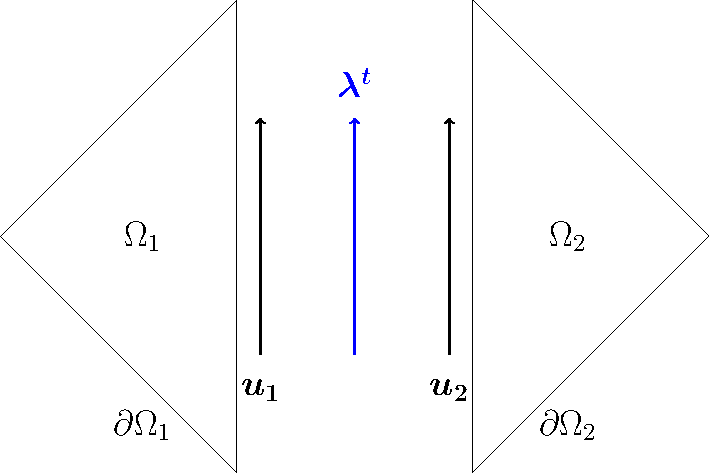
\includegraphics[scale=.5]{semi-hybrid-variables.pdf}}\hspace{2cm}
    \subfloat[\label{fig:double-hybrid-variables}]{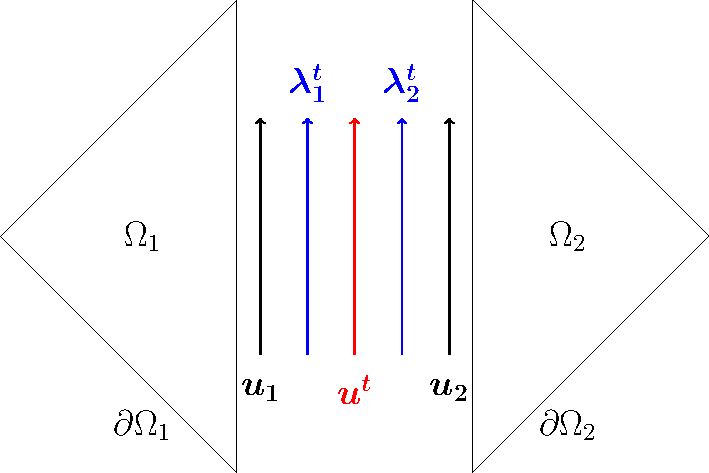
\includegraphics[scale=.5]{double-hybrid-variables.pdf}}\hfill
	\caption{Resulting variables for an internal interface shared by two adjacent elements using (a) Semi-hybrid and (b) hybrid-hybrid formulations. {\nathan Check if we are using lambdat}} {\giovane im gonna change this figure}
	\label{fig:hybrid-variables}
\end{figure}

Finally, the double-hybrid weak form searches for $\{\bm{u},p,\bm{t}^t,\bm{w}\} \in \mathcal{V}_D \times L^2 \times \bar{\mathcal{L}}^t \times \mathcal{W}_D$ such that:
\begin{subequations} \label{eq:double-hybrid-weak}
	\begin{align}
		a\left(\bm{u},\bm{v}\right)_{\mathcal{T}_h} - b\left( p, \bm{v}\right)_{\mathcal{T}_h} +\langle\bm{t}^t,\bm{v}\rangle_{\partial\mathcal{T}_h} &= \left(\bm{b},\bm{v}\right)_{\mathcal{T}_h} + \langle\bm{t}_N\cdot\bm{n},\bm{v}\cdot\bm{n}\rangle_{\partial\Omega_N} ~~\forall\, \bm{v} \in \mathcal{V}_0,\label{eq:double-hybrid-weak-a}\\ 
		-b\left(\bm{u}, q\right)_{\mathcal{T}_h} - c\left(p,q \right)_{\mathcal{T}_h} &= 0 ~~\forall\, q \in L^2, \label{eq:double-hybrid-weak-b}\\
		\langle\bm{u},\bm{s}^t\rangle_{\partial\mathcal{T}_h} - \langle\bm{w},\bm{s}^t\rangle_{\Gamma_h} &= 0 ~~\forall\, \bm{s}^t \in \bar{\mathcal{L}}^t, \label{eq:double-hybrid-weak-c}\\
		-\langle\bm{t}^t,\bm{z}\rangle_{\Gamma_h} &= -\langle\bm{t}_N^t,\bm{z}\rangle_{\partial\Omega_N} ~~\forall\, \bm{z} \in \mathcal{W}_0, \label{eq:double-hybrid-weak-d}
	\end{align}
\end{subequations}

\noindent where $\bm{z} \in \mathcal{W}_0$ is the test function for the tangential displacement on the mesh skeleton and $\bm{t}_N^t= \bm{t}_N - ((\bm{t}\cdot\bm{n})\bm{n})$ is the tangential component of the prescribed surface traction on $\partial\Omega_N$. The new operators in the variational problem from Eq. \eqref{eq:double-hybrid-weak} are defined as 
\begin{equation*}
	\langle\bm{t}^t,\bm{v}\rangle_{\partial\mathcal{T}_h} = \sum_{K \in \mathcal{T}_h} \int_{\partial K} \bm{t}^t \cdot \bm{v} \, d\partial K , \hspace{1cm}
	\langle\bm{w},\bm{s}^t\rangle_{\Gamma_h} = \sum_{E \in \Gamma_h} \int_{E} \bm{w} \cdot \jump{\bm{s}^t} \, d\partial K.
\end{equation*}

Note that Eq. \eqref{eq:double-hybrid-weak-d} is introduced to enforce the compatibility of tangential tractions across $\mathring{\Gamma}_h$ and to enforce $\bm{t}^t\lvert_{\partial\Omega_N}=\bm{t}_N^t$ in a weak sense. Moreover, Equation \eqref{eq:double-hybrid-weak-c} is deliberately written to emphasize the symmetry between its second term on the left-hand side and the left-hand side of Equation \eqref{eq:double-hybrid-weak-d}. 

The equivalence of problems \eqref{eq:double-hybrid-weak} and \eqref{eq:semi-hybrid-weak} can be verified by setting $\bm{s}^t \in \mathcal{L}^t \subset \bar{\mathcal{L}}^t$, so that $\jump{\bm{s}^t}\lvert_E=0$. Consequently, the second term in the left-hand side of Eq. \eqref{eq:double-hybrid-weak-c} vanishes. Moreover, $\langle\bm{u},\bm{s}^t\rangle_{\partial\mathcal{T}_h}=\langle\bm{u},\bm{s}^t\rangle_{\Gamma_h}-\langle\bm{u}_D,\bm{s}^t\rangle_{\partial\Omega_D} \, \forall \, \bm{s}^t \in \mathcal{L}^t$, considering that $\langle\bm{t}^t,\bm{v}\rangle_{\partial\mathcal{T}_h} = \langle\bm{t}^t,\bm{v}\rangle_{\Gamma_h}$ since $\bm{v}=\bm{0}\lvert_{\partial\Omega_D}$, and recalling that Eq. \eqref{eq:double-hybrid-weak-d} is no longer needed as it enforces the continuity of the broken tangential tractions, the solution $\left\{\bm{u},p,\bm{t}^t \right\}$ of problem \eqref{eq:double-hybrid-weak} is numerically equivalent to $\left\{\bm{u},p,\bm{t}^t \right\}$ from problem \eqref{eq:semi-hybrid-weak}. Therefore, convergence rates and error estimates are inherited from the semi-hybrid formulation.

\subsubsection{Error analysis}

The error analysis of the double-hybrid formulation for the Stokes flow is presented in \cite{puga2025stable} as an extension of \cite{carvalho2024semi} using the semi-hybrid method. We consider a homogeneous problem with $\bm{b}=\bm{0}$ and pure Dirichlet boundaries, i.e. $\bm{u}_D=\bm{0}$ on $\partial\Omega$. Let $\bm{u}$ and $p$ denote the exact solutions for displacement and pressure, respectively, while their approximations, $\bm{u}_h \in \mathcal{V}_{h,k}$ and $p_h \in \mathcal{P}_{h,k}$, are defined over a mesh $\mathcal{T}_h$ with size $h$ and polynomial order $k$.

According to \cite{brezzi2005mixed}, the convergence rates of velocity and pressure approximations are intrinsically linked, making the choice of approximation spaces a crucial factor. Specifically, the convergence rate is determined by the lowest of the approximation orders associated with $\bm{u}_h \in \mathcal{V}_{h,k}$ and $p_h \in \mathcal{P}_{h,k}$, measured in the $H^1$ and $L^2$ norms, respectively. Moreover, when adjoint-consistent formulations are utilized, the convergence of the $L^2$-norm error of the displacement can be increased by one order.

As the continuity of the tangential component of the displacement is weakly enforced when using $\bm{u}_h \in \mathcal{V}_{h,k} \subset H(\text{div},\Omega)$, we can draw an analogy with Discontinuous Galerkin formulations featuring partial penalization, which assuming that the pair $\mathcal{V}_{h,k} \times \mathcal{P}_{h,k}$ is divergence-compatible and satisfies the inf-sup condition, Theorems 5.1 and 5.2 of \cite{wang2007new} yield the error estimate:
\begin{equation}
\|\mathbf{u} - \mathbf{u}_h\|_{1,h} + \|p - p_h\| \leq C \left\{ h^k \|\mathbf{u}\|_{k+1} + h^{k+1} \|p\|_{k+1} \right\},
\end{equation}

\noindent with $k$ referring to the displacement's polynomials order and $C$ is a constant independent of $h$. For bidimensional convex domains with elliptic regularity, the displacement error may exhibit improved convergence rate by the expression:
\begin{equation}
\|\mathbf{u} - \mathbf{u}_h\| \leq C \left\{ h^{k+1} \|\mathbf{u}\|_{k+1} + h^{k+2} \|p\|_{k+1} \right\}.
\end{equation}

\subsection{Discrete double-hybrid-mixed finite element formulation}

The aim is to construct FE discrete spaces $\mathcal{S}_{h,k}=\mathcal{V}_{h,k} \times \mathcal{P}_{h,k} \times \bar{\mathcal{L}}^t_{h,k} \times \mathcal{W}_{h,k}$ for the double-hybrid-mixed formulation \eqref{eq:double-hybrid-weak}, associated with the mesh partition $\mathcal{T}_h$ with characteristic size $h$ and polynomial degree $k$. For conveniente, the subindex $k$ may be dropped in some equations.

The discrete form of the Double Hybrid Mixed methodology is henceforth denoted as DHM-H(div)($\mathcal{S}_{h,k}$). It seeks for $\{\bm{u}_h,p_h,\bm{t}^t_h,\bm{w}_h\} \in \mathcal{S}_{h,k}$ such that:
\begin{subequations} \label{eq:double-hybrid-discrete}
	\begin{align}
		a\left(\bm{u}_h,\bm{v}\right)_{\mathcal{T}_h} - b\left( p_h, \bm{v}\right)_{\mathcal{T}_h} +\langle\bm{t}^t_h,\bm{v}\rangle_{\partial\mathcal{T}_h} &= \left(\bm{b},\bm{v}\right)_{\mathcal{T}_h} + \langle\bm{t}_N\cdot\bm{n},\bm{v}\cdot\bm{n}\rangle_{\partial\Omega_N} ~~\forall\, \bm{v} \in \mathcal{V}_{h,k},\label{eq:double-hybrid-discrete-a}\\ 
		-b\left(\bm{u}_h, q\right)_{\mathcal{T}_h} - c\left(p_h,q \right)_{\mathcal{T}_h} &= 0 ~~\forall\, q \in \mathcal{P}_{h,k}, \label{eq:double-hybrid-discrete-b}\\
		\langle\bm{u}_h,\bm{s}^t\rangle_{\partial\mathcal{T}_h} - \langle\bm{w}_h,\bm{s}^t\rangle_{\Gamma_h} &= 0 ~~\forall\, \bm{s}^t \in \bar{\mathcal{L}}^t_{h,k}, \label{eq:double-hybrid-discrete-c}\\
		-\langle\bm{t}^t_h,\bm{z}^t\rangle_{\Gamma_h} &= -\langle\bm{t}_N^t,\bm{z}^t\rangle_{\partial\Omega_N} ~~\forall\, \bm{z}^t \in \mathcal{W}_{h,k}. \label{eq:double-hybrid-discrete-d}
	\end{align}
\end{subequations}

According to the Brezzi's theory in \cite{girault2012finite,brezzi2012mixed,arnold1988new}, the FE spaces associated with each variable cannot be chosen arbitrarily. 

Assume the pressure space is discontinuous, i.e.:
\begin{equation}
	\mathcal{P}_{h,k}(\mathcal{T}_h) = \{q \, \in L^2(\Omega) ~\lvert~ q\lvert_K \in \mathbb{P}_k(K) ~:~ \forall K \in \mathcal{T}_h\}
\end{equation}

\noindent which admits the following decomposition $\mathcal{P}=\bar{\mathcal{P}} \oplus \mathcal{P}^\perp$, where $\bar{\mathcal{P}}$ stands for piecewise constant functions over $\mathcal{T}_h$ and $\mathcal{P}^\perp$ is the piecewise zero-mean functions over $\mathcal{T}_h$. An alternative technique to avoid the construction of pressure functions with vanishing mean isdiscussed in Section \ref{sec:static-condensation}. For a divergence-compatible FE pair $\mathcal{V}_h \times \mathcal{P}_h$ tipically used to approximate flux and pressure in Darcy mixed problems, the condition
\begin{equation*}
	\nabla \cdot \mathcal{V}_{h,k} \subseteq \mathcal{P}_{h,k}.
\end{equation*}
holds independently of the discretization parameters, and is known to satisfy the inf-sup condition in the absence of the tangential tractions present in Eq. \eqref{eq:double-hybrid-weak-a} \cite{carvalho2024semi}.

However, mathematically proving the trace compatibility required in $\langle\bm{s}^t,\bm{v}\rangle_{\partial\mathcal{T}_h}$ and $\langle\bm{z},\bm{s}^t\rangle_{\Gamma_h}$ is a challenging task. In \cite{carvalho2024semi}, the authors had numerically demonstrated that trace compatibility can be verified by ensuring that the divergence-free subspaces $\mathcal{Z}(0)_{h,k}=\left\{ \bm{v} \in \mathcal{V}_{h,k} ~;~b(q,\bm{v})=0, ~\forall~q \in \mathcal{P}_{h,k} \right\}$ have sufficient polynomial order to guarantee that
\begin{equation*}
	\text{rank}~ \bm{D}^T = \text{dim} ~\mathcal{L}^t_{h,k},
\end{equation*}

\noindent where $\bm{D}^T=[\langle\bm{s}^t,\bm{v}\rangle_{\partial\mathcal{T}_h}]$. {\giovane Checar essa parte Phil }Analogously, the compatibility between the tangential tractions and tangential displacement is verified by checking the condition
\begin{equation*}
	\text{rank}~ \bm{L}^T = \text{dim} ~\mathcal{W}_{h,k},
\end{equation*}

\noindent with $\bm{L}^T=[\langle\bm{z},\bm{s}^t\rangle_{\Gamma_h}]$. In practical terms, the trace compatibility is guaranteed by enriching the internal functions of $\mathcal{V}_{h,k}$, which shall be demonstrated numerically.

Let $\hat{K}$ be a reference element with usual shapes:
\begin{itemize}
	\item Triangular elements in 2D: $\hat{T}= \left\{ \bm{\xi} \in \mathbb{R}^2 ~:~ 0 \leq \xi_1 \leq 1, ~0 \leq \xi_2 \leq 1-\xi_1 \right\}$;
	\item Quadrilateral elements in 2D: $\hat{Q}= \left\{ \bm{\xi} \in \mathbb{R}^2 ~:~ -1 \leq \xi_1 \leq 1, ~-1 \leq \xi_2 \leq 1 \right\}$;
	\item Tetrahedral elements in 3D: $\hat{Te}= \left\{ \bm{\xi} \in \mathbb{R}^3 ~:~ 0 \leq \xi_1 \leq 1, ~0 \leq \xi_2 \leq 1-\xi_1, ~0 \leq \xi_3 \leq 1-\xi_1-\xi_2 \right\}$;
	\item Hexahedral elements in 3D: $\hat{H}= \left\{ \bm{\xi} \in \mathbb{R}^3 ~:~ -1 \leq \xi_1 \leq 1, ~-1 \leq \xi_2 \leq 1, ~-1 \leq \xi_3 \leq 1 \right\}$.
\end{itemize}

The finite subspaces $\mathcal{V}_{h,k}(\hat{K})$ and $\mathcal{P}_{h,k}(\hat{K})$ are divergence-compatible polynomial spaces, so that $\nabla \cdot \mathcal{V}_{h,k}(\hat{K}) = \mathcal{P}_{h,k}(\hat{K})$. The elements $K \in \mathcal{T}_h$ are mapped from the adimensional space by $\mathcal{F}: \hat{K}\rightarrow K$. For scalar functions, 
\begin{equation*}p \in \mathcal{P}_{h,k}(K):p=\mathcal{F}(\hat{p}) = \hat{p}\,\circ\,\mathcal{F}^{-1}, \, \hat{p} \in \mathcal{P}_{h,k}(\hat{K}).	
\end{equation*}

For vector-valued functions, the isomorphism $L^2(\hat{K})$ to $L^2(K)$ defined for scalar functions does not preserve the continuity of the normal component over the deformed element $K$, so the Piola transformation is used instead: 
\begin{equation} \label{eq:piola-transform}
\bm{v} \in \mathcal{V}_{h,k}(K): \bm{v}=\bar{\mathcal{F}}(\bm{\hat{v}})=\left[\frac{1}{J}\nabla\mathcal{F}\bm{\hat{v}} \right] \,\circ\, \mathcal{F}^{-1}, \, \bm{\hat{v}} \in \mathcal{V}_{h,k}(\hat{K}), 
\end{equation}

\noindent where $\nabla\mathcal{F}$ is the Jacobian matrix of the transformation $\mathcal{F}$ and $J=\lvert\text{det}(\nabla\mathcal{F})\lvert$. It direct follows from Eq. \eqref{eq:piola-transform} that $\nabla \cdot \bar{\mathcal{F}}(\bm{\hat{v}})=\frac{1}{J} \hat{\nabla} \cdot \bm{\hat{v}}$. The same transformation is valid for vector functions $\bm{s}^t \in \bar{\mathcal{L}}_{h,k}(\partial K): \bm{s}^t=\bar{\mathcal{F}}(\bm{\hat{s}}^t)$ and $\bm{z} \in \mathcal{W}_{h,k}(E): \bm{z}=\bar{\mathcal{F}}(\bm{\hat{z}})$ defined over the mesh skeleton. Additionally, the displacement space admits a decomposition $\mathcal{V}_{h,k}=\mathcal{V}^\partial_{h,k} \oplus \mathring{\mathcal{V}}_{h,k}$ in terms of functions with continuous normal components over $\partial\hat{K}$, $\mathcal{V}^\partial_{h,k}$, and the ones with vanishing trace over $\partial\hat{K}$, $\mathring{\mathcal{V}}_{h,k}$.

The construction of the divergence-compatible spaces adopted in this work is better detailed in \cite{de2013new,devloo2022efficient}, and some classic stable pairs are depicted in Table \ref{tab:FE_pairs} for the element shapes described above. The notation adopted is as follows: $\mathbb{P}_k(\hat{K})$ stands for scalar polynomials of total degree at most $k$, $\tilde{\mathbb{P}}_k(\hat{K})=\left\{\mathbb{P}_k(\hat{K}) ~:~\mathbb{P}_k\lvert_{\partial\hat{K}}=0 \right\}$ its the homogeneous set and $\mathbb{P}_k(\hat{K},\mathbb{R}^d)$ is their respective vectorial counterpart. $\mathbb{Q}_{k,m}(\hat{K})$ and $\mathbb{Q}_{k,m,n}(\hat{K})$ refer to the polynomials with maximum degree order $k,m$ or $n$ in each direction, respectively.

\begin{table}[h]
    \centering
    \renewcommand{\arraystretch}{1.5}
    \begin{tabular}{c l c c}
        \toprule
        $\bm{\hat{K}}$ & \textbf{Method} & $\bm{\mathcal{V}(\hat{K})}$ & $\bm{\mathcal{P}(\hat{K})}$ \\
        \midrule
        \multirow{3}{*}{$\hat{T}$} 
        & $BDM(k)^{\text{\cite{brezzi1985two}}}$ & $\mathbb{P}_k(\hat{K}, \mathbb{R}^2)$ & $\mathbb{P}_{k-1}(\hat{K})$ \\
        & $RT(k)^{\text{\cite{arnold1990mixed}}}$ & $\mathbb{P}_k(\hat{K}, \mathbb{R}^2) \oplus \mathbf{x} \tilde{\mathbb{P}}_k(\hat{K})$ & $\mathbb{P}_k(\hat{K})$ \\
        & $BDM^+(k)^{\text{\cite{brezzi2012mixed}}}$ & $\mathbb{P}_k^{\partial}(\hat{K}, \mathbb{R}^2) \oplus \mathring{\mathbb{P}}_{k+1}(\hat{K}, \mathbb{R}^2)$ & $\mathbb{P}_k(\hat{K})$ \\
        \midrule
        \multirow{2}{*}{$\hat{R}$} 
        & $RT(k)^{\text{\cite{arnold1990mixed}}}$ & $\mathbb{Q}_{k+1,k} \times \mathbb{Q}_{k,k+1}(\hat{K})$ & $\mathbb{Q}_{k,k}(\hat{K})$ \\
        & $RT^+(k)^{\text{\cite{farias2017two}}}$ & $\mathcal{V}_{RT(k)}^\partial(\hat{K}) \oplus \mathring{\mathcal{V}}_{RT(k+1)}(\hat{K})$ & $\mathbb{Q}_{k+1,k+1}(\hat{K})$ \\
        \midrule
        \multirow{3}{*}{$\hat{Te}$} 
        & $BDM(k)^{\text{\cite{brezzi1987mixed}}}$ & $\mathbb{P}_k(\hat{K}, \mathbb{R}^3)$ & $\mathbb{P}_{k-1}(\hat{K})$ \\
        & $RT(k)^{\text{\cite{nedelec1980mixed}}}$ & $\mathbb{P}_k(\hat{K}, \mathbb{R}^3) \oplus \mathbf{x} \tilde{\mathbb{P}}_k(\hat{K})$ & $\mathbb{P}_k(\hat{K})$ \\
        & $BDM^+(k)^{\text{\cite{brezzi2012mixed}}}$ & $\mathbb{P}_k^\partial(\hat{K}, \mathbb{R}^3) \oplus \mathring{\mathbb{P}}_{k+1}(\hat{K}, \mathbb{R}^3)$ & $\mathbb{P}_k(\hat{K})$ \\
        \midrule
        \multirow{2}{*}{$\hat{H}$} 
        & $RT(k)^{\text{\cite{nedelec1980mixed}}}$ & $\mathbb{Q}_{k+1,k,k} \times \mathbb{Q}_{k,k+1,k} \times \mathbb{Q}_{k,k,k+1}(\hat{K})$ & $\mathbb{Q}_{k,k,k}(\hat{K})$ \\
        & $RT^+(k)^{\text{\cite{castro2016hierarchical}}}$ & $\mathcal{V}_{RT(k)}^\partial(\hat{K}) \oplus \mathring{\mathcal{V}}_{RT(k+1)}(\hat{K})$ & $\mathbb{Q}_{k+1,k+1,k+1}(\hat{K})$ \\
        \bottomrule
    \end{tabular}
    \caption{Examples of divergence-compatible pairs $\mathcal{V}(\hat{K}) \times \mathcal{P}(\hat{K})$ in the reference element for displacement and pressure fields \cite{carvalho2024semi}.}
    \label{tab:FE_pairs}
\end{table}

On top of that, let us adopt vector-valued polynomial spaces for the Lagrange multipliers $\bm{\hat{t}}^t \in \bar{\mathcal{L}}(\partial \hat{K})$ and $\bm{\hat{w}} \in \mathcal{W}(\hat{E})$, to be combined with the divergence-compatible $\mathcal{V}(\hat{K})\times\mathcal{P}(\hat{K})$:
\begin{itemize}
	\item For 1D segments: $\bar{\mathcal{L}}(\partial \hat{K})=\mathbb{P}_m(\partial \hat{K})\bm{\tau}^{\partial\hat{K}}$ and $\mathcal{W}(\hat{E})=\mathbb{P}_m(\hat{E})\bm{\tau}^{\hat{E}}$;
	\item For triangular facets: $\bar{\mathcal{L}}(\partial \hat{K})=\bm{\hat{n}} \wedge \mathbb{P}_m(\partial \hat{K},\mathbb{R}^3)$ and $\mathcal{W}(\hat{E})=\bm{\hat{n}} \wedge \mathbb{P}_m(\hat{E},\mathbb{R}^3)$;
	\item For quadrilateral facets: $\bar{\mathcal{L}}(\partial \hat{K})=\bm{\hat{n}} \wedge \mathbb{Q}_{m,m}(\partial \hat{K},\mathbb{R}^3)$ and $\mathcal{W}(\hat{E})=\bm{\hat{n}} \wedge \mathbb{Q}_{m,m}(\hat{E},\mathbb{R}^3)$.
\end{itemize}

\noindent In the above expressions, $\bm{\tau}^{\partial\hat{K}}$ and $\bm{\tau}^{\hat{E}}$ are the tangential vectors to the line segment, unique for $\hat{E}$ and a pair with opposite directions for $\partial\hat{K}$, and $\wedge$ stands for the wedge product. The order $m$ is not arbitrary, instead it has to be chosen accordingly to ensure the trace compatibility between the discrete spaces shown in Table \ref{tab:FE_pairs}. {\giovane Devemos fazer uma analise com diferentes valores de m para verificar a compatibilidade do traco?}

\subsection{Comparison with H1-hybrid formulation}

{\giovane O Phil trabalhou nisso na China, talvez ele poderia escrever essa parte?}

\subsection{Static condensation procedure} \label{sec:static-condensation}

Solving the problem of Equation \eqref{eq:double-hybrid-discrete} as presented would demand significantly more computational efforts compared to traditional $H^1$ primal methods or even with mixed Taylor-Hood approximations. First, the divergence-compatible pair $\mathcal{V}_{h,k} \times \mathcal{P}_{h,k}$ includes a larger number of functions for a given polynomial order $k$ than the traditional $H^1$ subspaces. Second, the introduction of Lagrange multipliers due to hybridization not only increase the number of unknowns but also leads to a a more challenging saddle-point problem. Moreover, {\nathan some of?} the advantages of the DHM-H(div) formulation only appear after applying the static condensation procedure, as shall be demonstrated next.

Hybridization techniques have been widely used in the literature {\nathan if you state this, you should include citations} along with static condensation to reduce the size of global system to be solved. The procedure consists on separating the global degrees of freedom (DOFs) into two sets: one containing the DOFs that are possible to be solved within a single element, called internal DOFs, and the other containing the DOFs that are shared between elements and therefore cannot be solved locally, called external (or main) DOFs. {\nathan should we cite TNDSS here or in the introduction?}

As previously mentioned, the displacement functions $\bm{u}_h \in \mathcal{V}_{h,k}$ can be separated into element-wise divergence-free functions with vanishing normal components over the element boundaries, namely $\mathring{\bm{u}}_h$, and the remaining functions with continuous normal components across elements boundaries, $\bm{u}^\partial_h$. This leads to the definition of two auxiliary spaces, namely:
\begin{subequations} \label{eq:internal-external-functions}
	\begin{align}
		\mathring{\mathcal{V}}_{h,k}(K,\mathbb{R}^d) &= \left\{ \bm{v} \in \mathcal{V}_{h,k}(K,\mathbb{R}^d) ~:~ \int_K\nabla \cdot \bm{v}\,dK = 0, ~\bm{v}\cdot\bm{n}\lvert_{\partial K} = 0 \right\},\\
		\mathcal{V}^\partial_{h,k}(K,\mathbb{R}^d) &= \left\{ \bm{v} \in \mathcal{V}_{h,k}(K,\mathbb{R}^d) ~:~ \nabla \cdot \bm{v} \subset \mathcal{P}_{h,k}(K) ~:~ \bm{v}\cdot\bm{n}\lvert_{\partial K} \neq 0 \right\}.
	\end{align}
\end{subequations}

The element-wise divergence-free functions can be classified as internal functions because they do not contribute to the pure dilation and compression deformation modes that could affect multiple elements.

To avoid constructing a pressure space $\mathcal{P}_{h,k}$ that includes both piecewise constant and piecewise zero-mean functions, two additional variables can be added to the problem, namely the elemental average pressure $\bar{p}_h \in \bar{\mathcal{P}}_h$ and the distributed force $g_h \in \bar{\mathcal{P}}_{h}$. This approach enables not only the construction of $\mathcal{P}_{h,k}$ using traditional piecewise polynomials of order $k$ but also the condensation of all the higher-order pressure functions. It is worth mentioning that for compressible solids, the pressure can be computed explicitly from the displacement, making these two additional spaces no longer necessary.

Under these assumptions, the DHM-H(div)($\mathcal{S}_{h,k}$) can be written as: find $\{\bm{u}^\partial_h,\mathring{\bm{u}}_h,p_h,\bm{t}^t_h,\bm{w}_h,\bar{p}_h,\bar{g}_h\} \in \{\mathcal{V}^\partial_h \times \mathring{\mathcal{V}}_h \times \mathcal{P}_h \times \bar{\mathcal{L}}_h \times \mathcal{W}_h \times \bar{\mathcal{P}} \times \bar{\mathcal{P}} \}$ such that:
\begin{subequations} \label{eq:double-hybrid-six-field}
	\begin{align}
		a(\bm{u}^\partial_h,\bm{v}^\partial)_{\mathcal{T}_h} + a(\mathring{\bm{u}}_h,\bm{v}^\partial)_{\mathcal{T}_h} - b( p_h, \bm{v}^\partial)_{\mathcal{T}_h} +\langle\bm{t}^t_h,\bm{v}^\partial\rangle_{\partial\mathcal{T}_h} &= (\bm{b},\bm{v}^\partial)_{\mathcal{T}_h} + \langle\bm{t}_N\cdot\bm{n},\bm{v}^\partial\cdot\bm{n}\rangle_{\partial\Omega_N}, \label{eq:double-hybrid-six-field-a}\\
		a(\bm{u}^\partial_h,\mathring{\bm{v}}_h)_{\mathcal{T}_h} + a(\mathring{\bm{u}}_h,\mathring{\bm{v}}_h)_{\mathcal{T}_h} - b( p_h, \mathring{\bm{v}}_h)_{\mathcal{T}_h} +\langle\bm{t}^t_h,\mathring{\bm{v}}_h\rangle_{\partial\mathcal{T}_h} &= (\bm{b},\mathring{\bm{v}}_h)_{\mathcal{T}_h} + \langle\bm{t}_N\cdot\bm{n},\mathring{\bm{v}}_h\cdot\bm{n}\rangle_{\partial\Omega_N}, \label{eq:double-hybrid-six-field-b}\\ 
		-b(\bm{u}^\partial_h, q)_{\mathcal{T}_h} - b(\mathring{\bm{u}}_h, q)_{\mathcal{T}_h} - c(p_h,q)_{\mathcal{T}_h} + (\bar{g}_h,q) &= 0, \label{eq:double-hybrid-six-field-c}\\
		\langle\bm{u}^\partial_h,\bm{s}^t\rangle_{\partial\mathcal{T}_h} + \langle\mathring{\bm{u}}_h,\bm{s}^t\rangle_{\partial\mathcal{T}_h} - \langle\bm{w}_h,\bm{s}^t\rangle_{\Gamma_h} &= 0, \label{eq:double-hybrid-six-field-d}\\
		-\langle\bm{t}^t_h,\bm{z}\rangle_{\Gamma_h} &= -\langle\bm{t}_N^t,\bm{z}\rangle_{\partial\Omega_N}, \label{eq:double-hybrid-six-field-e}\\
		(p_h-\bar{p}_h,\bar{\rho})_{\mathcal{T}_h} &= 0, \label{eq:double-hybrid-six-field-f}\\
		-(\bar{g}_h,\bar{q})_{\mathcal{T}_h} &= 0, \label{eq:double-hybrid-six-field-g}
	\end{align}
\end{subequations}

\noindent for all$\{\bm{v}^\partial,\mathring{\bm{v}}, q, \bm{s}^t, \bm{z}, \bar{\rho}, \bar{q} \} \in \{\mathcal{V}^\partial_{h,k} \times \mathring{\mathcal{V}}_{h,k} \times \mathcal{P}_{h,k} \times \bar{\mathcal{L}}^t_{h,k} \times \mathcal{W
}_{h,k} \times \bar{\mathcal{P}} \times \bar{\mathcal{P}}\}$.

The definition of $\mathcal{V}^\partial \text{ and } \mathring{\mathcal{V}}$ in Eq. \eqref{eq:internal-external-functions} directly implies that the terms $\langle\bm{t}^t_h,\bm{v}^\partial\rangle_{\partial\mathcal{T}_h}, b( p_h, \mathring{\bm{v}}_h)_{\mathcal{T}_h}, \langle\bm{t}_N\cdot\bm{n},\mathring{\bm{v}}_h\cdot\bm{n}\rangle_{\partial\Omega_N} \text{ and }\langle\bm{u}^\partial_h,\bm{s}^t\rangle_{\partial\mathcal{T}_h}$ vanish. Recalling that $\bm{t}^t \in \bar{\mathcal{L}}_{h,k}$ is discontinuous over the mesh sleleton, meaning that it can be computed from a single element in the mesh, the problem of Eq. \eqref{eq:double-hybrid-six-field} can be rearranged in matrix form as:
\vspace{0.8cm}
\begin{equation} \label{eq:block-matrix}
	\begin{bNiceArray}{c | c}[cell-space-top-limit=10pt,cell-space-bottom-limit=10pt,extra-margin=5pt]
		\begin{bmatrix}
			\bm{A}_{\smallcirc\smallcirc} & \bm{0} & \bm{D} & 0 \\
			\bm{0} & \bm{C} & \bm{0} & \bm{M} \\
			\bm{D}^T & \bm{0} & \bm{0} & \bm{0} \\
			\bm{0} & \bm{M}^T & \bm{0} & \bm{0}
			\end{bmatrix}
			&
			\begin{bmatrix}
			\bm{A}_{\partial\smallcirc} & \bm{0} & \bm{0} \\
			\bm{B} & \bm{0} & \bm{0} \\
			\bm{0} & \bm{L} & \bm{0} \\
			\bm{0} & \bm{0} & \bm{G}
			\end{bmatrix}
			\\ \hline
			\begin{bmatrix}
			\bm{A}_{\smallcirc\partial} & \bm{B}^T & \bm{0} & \bm{0} \\
			\bm{0} & \bm{0} & \bm{L}^T & \bm{0} \\
			\bm{0} & \bm{0} & \bm{0} & \bm{G}^T \\
			\end{bmatrix}
			&
			\begin{bmatrix}
			\bm{A}_{\partial\partial} & \bm{0} & \bm{0} \\
			\bm{0} & \bm{0} & \bm{0} \\
			\bm{0} & \bm{0} & \bm{0}
			\end{bmatrix}
			\CodeAfter
			\OverBrace[shorten,yshift=5pt]{1-1}{2-1}{\bm{K}_{ii}}
			\OverBrace[shorten,yshift=5pt]{1-2}{2-2}{\bm{K}_{ie}}
			\UnderBrace[shorten,yshift=5pt]{1-1}{2-1}{\bm{K}_{ei}}
			\UnderBrace[shorten,yshift=5pt]{1-2}{2-2}{\bm{K}_{ee}}
	\end{bNiceArray}
	\begin{BNiceArray}{c}[cell-space-top-limit=10pt,cell-space-bottom-limit=10pt,extra-margin=5pt]
		\begin{Bmatrix}
			\mathring{\bm{u}} \\
			p \\
			\bm{t}^t \\
			\bar{g}
		\end{Bmatrix}
		\\ \hline
		\begin{Bmatrix}
			\bm{u}^\partial \\
			\bm{w} \\
			\bar{p}
		\end{Bmatrix}
		\CodeAfter
		\OverBrace[shorten,yshift=5pt]{1-1}{2-1}{\bm{\alpha}_{i}}
		\UnderBrace[shorten,yshift=5pt]{1-1}{2-1}{\bm{\alpha}_{e}}
	\end{BNiceArray}
	=
	\begin{BNiceArray}{c}[cell-space-top-limit=10pt,cell-space-bottom-limit=10pt,extra-margin=5pt]
		\begin{Bmatrix}
			\mathring{\bm{f}} \\
			0 \\
			0 \\
			0
		\end{Bmatrix}
		\\
		\begin{Bmatrix}
			\bm{f}^\partial\\
			\bm{f}^t \\
			0
		\end{Bmatrix}
		\CodeAfter
		\OverBrace[shorten,yshift=5pt]{1-1}{2-1}{\bm{f}_{i}}
		\UnderBrace[shorten,yshift=5pt]{1-1}{2-1}{\bm{f}_{e}}
	\end{BNiceArray},
\end{equation}
\vspace{0.6cm}

\noindent where $\bm{\alpha}_i=\{\mathring{\bm{u}},p,\bm{t}^t,\bar{g}\}$ and $\bm{\alpha}_e=\{\bm{u}^\partial,\bm{w},\bar{p}\}$ are the sets containing the internal and external degrees of freedom, respectively. Each block matrix is associated with the following operators:
\begin{equation}
	\begin{aligned}
		\bm{A}_{\smallcirc\smallcirc} &= \sum_{K \in \mathcal{T}_h} \int_{K} \bm{\varepsilon}(\mathring{\bm{v}}) : \mathcal{D}^{'} : \bm{\varepsilon}(\mathring{\bm{u}}) dK , &\bm{A}_{\smallcirc\partial} &= \sum_{K \in \mathcal{T}_h} \int_{K} \bm{\varepsilon}(\mathring{\bm{v}}) : \mathcal{D}^{'} : \bm{\varepsilon}(\bm{u}^\partial) dK ,\\
		\bm{A}_{\partial\smallcirc} &= \sum_{K \in \mathcal{T}_h} \int_{K} \bm{\varepsilon}(\bm{v}^\partial) : \mathcal{D}^{'} : \bm{\varepsilon}(\mathring{\bm{u}}) dK , &\bm{A}_{\partial\partial} &= \sum_{K \in \mathcal{T}_h} \int_{K} \bm{\varepsilon}(\bm{v}^\partial) : \mathcal{D}^{'} : \bm{\varepsilon}(\bm{u}^\partial) dK ,\\
		\bm{B} &= \sum_{K \in \mathcal{T}_h} -\int_{K} p \,\nabla \cdot \bm{v}^\partial \, dK , & \bm{C} &= \sum_{K \in \mathcal{T}_h} -\int_{K} \frac{1}{\kappa} \,p \,q \, dK ,\\
		\bm{D} &= \sum_{K \in \mathcal{T}_h} \int_{\partial K} \bm{t}^t \cdot \mathring{\bm{v}} \, d\partial K , &\bm{G} &= \sum_{K \in \mathcal{T}_h} -\int_{K} \bar{p} \, \bar{\rho} \, dK ,\\
		\bm{L} &= \sum_{E \in \Gamma_h} -\int_{E} \bm{w} \cdot \jump{\bm{s}^t} \, d\partial K , &\bm{M} &= \sum_{K \in \mathcal{T}_h} \int_{K} \bar{g} \, q \, dK .
	\end{aligned}
\end{equation}

Writing Eq. \eqref{eq:block-matrix} in a compact form yields
\begin{equation} \label{eq:compact-form}
	\begin{bmatrix}
		\bm{K}_{ii} & \bm{K}_{ie} \\
		\bm{K}_{ei} & \bm{K}_{ee}
	\end{bmatrix}
	\begin{Bmatrix}
		\bm{\alpha}_i \\
		\bm{\alpha}_e
	\end{Bmatrix}
	=
	\begin{Bmatrix}
		\bm{f}_i \\
		\bm{f}_e
	\end{Bmatrix},
\end{equation}

\noindent so the static condensation is performed by eliminating the internal variables as follows:
\begin{equation} \label{eq:static-condensation}
	\begin{aligned}
		\bar{\bm{K}} &= \bm{K}_{ee} - \bm{K}_{ei}\bm{K}_{ii}^{-1}\bm{K}_{ie},\\
		\bar{\bm{f}} &= \bm{f}_e - \bm{K}_{ei}\bm{K}_{ii}^{-1}\bm{f}_i,
	\end{aligned}
\end{equation}

\noindent resulting in the reduced linear system:
\begin{equation} \label{eq:reduced-linear-system}
	\bar{\bm{K}}\bm{\alpha}_e = \bar{\bm{f}}.
\end{equation}

\noindent The internal variables are then recovered in a post-processing step by solving a local problem at the element level: $\bm{\alpha}_i = \bm{K}_{ii}^{-1}(\bm{f}_i - \bm{K}_{ie}\bm{\alpha}_e)$.

To better analyze the spectral properties of the resulting matrix, let us break through the static condensation procedure step by step. The Lagrange multiplier $\bm{w}$, representing the tangential velocities, only has coupling terms with the tangent tractions by the matrix $\bm{L}$. Therefore, matrix $\bm{A}_{\smallcirc\smallcirc}$ is positive definite. Proceeding by statically condensing the internal displacements onto the tangential tractions $\bm{t}^t$ leads to:
\begin{equation} \label{eq:block-matrix-1}
	\begin{NiceArray}{l}[cell-space-top-limit=2pt,cell-space-bottom-limit=2pt,extra-margin=4pt]
			p \\
			\bm{t}^t \\
			\bar{g} \\
			\bm{u}^\partial \\
			\bm{w} \\
			\bar{p} 
	\end{NiceArray}
	\begin{bNiceArray}{c c c | c c c}[cell-space-top-limit=2pt,cell-space-bottom-limit=2pt,extra-margin=2pt]
			\bm{C} & \bm{0} & \bm{M} & \bm{B} & \bm{0} & \bm{0} \\
			\bm{0} & -\bm{D}\bm{A}_{\smallcirc\smallcirc}^{-1}\bm{D}^T & \bm{0} & -\bm{D}\bm{A}_{\smallcirc\smallcirc}^{-1}\bm{A}_{\partial\smallcirc} & \bm{L} & \bm{0} \\
			\bm{M}^T & \bm{0} & \bm{0} & \bm{0} & \bm{0} & \bm{G}
			\\ \hline
			\bm{B}^T & -\bm{A}_{\smallcirc\partial}\bm{A}_{\smallcirc\smallcirc}^{-1}\bm{D}^T & \bm{0} & \bm{A}_{\partial\partial} & \bm{0} & \bm{0} \\
			\bm{0} & \bm{L}^T & \bm{0} & \bm{0} & \bm{0} & \bm{0} \\
			\bm{0} & \bm{0} & \bm{G}^T & \bm{0} & \bm{0} & \bm{0}
	\end{bNiceArray}
	\Leftrightarrow
	\begin{bNiceArray}{c c c | c c c}[cell-space-top-limit=2pt,cell-space-bottom-limit=2pt,extra-margin=2pt]
		\bm{C} & \bm{0} & \bm{M} & \bm{B} & \bm{0} & \bm{0} \\
		\bm{0} & -\bar{\bm{A}}_{\smallcirc\smallcirc} & \bm{0} & \bar{\bm{D}} & \bm{L} & \bm{0} \\
		\bm{M}^T & \bm{0} & \bm{0} & \bm{0} & \bm{0} & \bm{G}
		\\ \hline
		\bm{B}^T & \bar{\bm{D}}^T & \bm{0} & \bm{A}_{\partial\partial} & \bm{0} & \bm{0} \\
		\bm{0} & \bm{L}^T & \bm{0} & \bm{0} & \bm{0} & \bm{0} \\
		\bm{0} & \bm{0} & \bm{G}^T & \bm{0} & \bm{0} & \bm{0}
\end{bNiceArray},
\end{equation}

\noindent where $\bar{\bm{A}}_{\smallcirc\smallcirc}=\bm{D}\bm{A}_{\smallcirc\smallcirc}^{-1}\bm{D}^T$ and $\bar{\bm{D}}=-\bm{D}\bm{A}_{\smallcirc\smallcirc}^{-1}\bm{A}_{\partial\smallcirc}$. The matrix $\bar{\bm{A}}_{\smallcirc\smallcirc}$ is symmetric positive definite if the spaces $\mathcal{V}_{h}$ and $\bar{\mathcal{L}}_{h}$ are trace compatible. In other words, this condition holds if the number of internal shape functions in the displacement space is sufficiently large compared to the number of tangential traction functions. For the numeric examples presented in Section \ref{sec:Examples}, the polynomial order of the internal displacement functions is three orders higher than the polynomial order of the tangential traction functions.

The tangential tractions $\bm{t}^t$ in Eq. \eqref{eq:block-matrix-1} can be condensed onto the tangential velocities $\bm{w}$, yielding
\begin{equation} \label{eq:block-matrix-2}
	\begin{NiceArray}{l}[cell-space-top-limit=2pt,cell-space-bottom-limit=2pt,extra-margin=4pt]
		p \\
		\bar{g} \\
		\bm{u}^\partial \\
		\bm{w} \\
		\bar{p} 
	\end{NiceArray}
\begin{bNiceArray}{c c | c c c}[cell-space-top-limit=2pt,cell-space-bottom-limit=2pt,extra-margin=2pt]
	\bm{C} & \bm{M} & \bm{B} & \bm{0} & \bm{0} \\
	\bm{M}^T & \bm{0} & \bm{0} & \bm{0} & \bm{G}
	\\ \hline
	\bm{B}^T & \bm{0} & \bm{A}_{\partial\partial} & \bm{L}\bar{\bm{A}}_{\smallcirc\smallcirc}^{-1}\bar{\bm{D}} & \bm{0} \\
	\bm{0} & \bm{0} & \bar{\bm{D}}^T\bar{\bm{A}}_{\smallcirc\smallcirc}^{-1}\bm{L}^T & \bm{L}\bar{\bm{A}}_{\smallcirc\smallcirc}^{-1}\bm{L}^T & \bm{0} \\
	\bm{0} & \bm{G}^T & \bm{0} & \bm{0} & \bm{0}
\end{bNiceArray}
\Leftrightarrow
\begin{bNiceArray}{c c | c c c}[cell-space-top-limit=2pt,cell-space-bottom-limit=2pt,extra-margin=2pt]
	\bm{C} & \bm{M} & \bm{B} & \bm{0} & \bm{0} \\
	\bm{M}^T & \bm{0} & \bm{0} & \bm{0} & \bm{G}
	\\ \hline
	\bm{B}^T & \bm{0} & \bm{A}_{\partial\partial} & \bm{A}_{\partial\smallcirc}^* & \bm{0} \\
	\bm{0} & \bm{0} & \bm{A}_{\smallcirc\partial}^* & \bm{A}_{\smallcirc\smallcirc}^* & \bm{0} \\
	\bm{0} & \bm{G}^T & \bm{0} & \bm{0} & \bm{0}
\end{bNiceArray},
\end{equation}

\noindent where $\bm{A}_{\smallcirc\smallcirc}^*=\bm{L}\bar{\bm{A}}_{\smallcirc\smallcirc}^{-1}\bm{L}^T$ and $\bm{A}_{\partial\smallcirc}^*=\bm{L}\bar{\bm{A}}_{\smallcirc\smallcirc}^{-1}\bar{\bm{D}}$. The matrix $\bm{A}_{\smallcirc\smallcirc}$ is symmetric positive definite because the number of functions approximating the tangential displacements within the block $\bm{L}$ matches exactly the number of tangential traction functions \cite{puga2025stable}. The static condensation procedure can be further applied to eliminate $p \text{ and } \bar{g}$, leading to the following matrix structure:
\begin{equation} \label{eq:block-matrix-3}
	\begin{NiceArray}{l}[cell-space-top-limit=2pt,cell-space-bottom-limit=2pt,extra-margin=4pt]
		\bm{u}^\partial \\
		\bm{w} \\
		\bar{p} 
	\end{NiceArray}
\begin{bNiceArray}{c c c}[cell-space-top-limit=2pt,cell-space-bottom-limit=2pt,extra-margin=2pt]
	\bm{A}_{\partial\partial} & \bm{A}_{\partial\smallcirc}^* & \bar{\bm{B}} \\
	\bm{A}_{\smallcirc\partial}^* & \bm{A}_{\smallcirc\smallcirc}^* & \bm{0} \\
	\bar{\bm{B}}^T & \bm{0} & \bm{0}
\end{bNiceArray}.
\end{equation}

As a consequence of this procedure, a symmetric positive-definite matrix is obtained for a compressible solid with two unknowns, $\{\bm{u}^\partial_h,\bm{w}\} \in \mathcal{V}^\partial \times \mathcal{W}$. In this case, the block matrix $\bm{C}$ is positive definite, allowing it to be condensed without the need of introducing $\bar{p}$ and $\bar{g}$. For the incompressible case, where pressures cannot be explicitly computed from the displacements, a single mean pressure per element $\bar{p}_h \in \bar{\mathcal{P}}$ acts as a Lagrange multiplier in the global system. This results in a saddle-point matrix, but with improved spectral properties and easier to solve compared to Eqs. \eqref{eq:semi-hybrid-weak-a}-\eqref{eq:semi-hybrid-weak-c}.

\section{Examples \label{sec:Examples}}

In this section, the proposed methodology is tested and verified through three benchmarks for which analytical and/or numerical solutions are available and a real-world problem. In the first case, a non-homogeneous solid under pure stretch is analyzed to show the advantage of the hybrid formulation to represent stress discontinuities over element interfaces in comparison to the Taylor-Hood scheme. In the second example, a cantilever beam is investigated in different compressibility regime to show the independency of the convergence rate to the poisson coefficient. Next, the classical Cook's membrane problem is solved, followed by a real-world problem where the applicability of the method is demonstrated.

\subsection{Uniform stretch of a non-homogeneous solid \label{subsec:non-homogeneous}}

As a first example, a simple uniform stretch test of a heterogeneous cube specimen is studied. The domain is $\Omega=[0,1] \times [0,1] \times [0,1]$ composed of two horizontal layers with equal Poisson coefficient $\nu$ and different Young modulus, namely $E^1$ and $E^2$, according to Figure \ref{fig:non-homogeneous-stretch-geometry}. The analytic solution for this problem is easily obtained from the linear elasticity theory, where the stresses are:
\begin{equation}
	\begin{aligned}
		p^i &= -\frac{(2-2 \nu ) E^i}{6 (\nu +1)}-\frac{2 \nu 
		E^i}{3 (\nu +1)}, \\
		\sigma^i_{xx} &= \frac{2(1-\nu)E^i}{2(1+\nu)}-\frac{\nu E^i}{3(1+\nu)}, \\
		\sigma^i_{yy} &= 0, \\
		\sigma^i_{zz} &= \frac{\nu E^i}{\nu +1}, \\
		\sigma_{xy} &= \sigma_{xz} = \sigma_{yz} = 0,
	\end{aligned}
\end{equation}

\noindent with the superscript $(\cdot)^i$ standing for the $i$-th material. The displacements solution is given by:
\begin{equation}
	\begin{aligned}
		u_x &= (1-\nu)x, \\
		u_y &= -\nu y, \\
		u_z &= 0.
	\end{aligned}
\end{equation}

\begin{figure}[!htb]
    \centering
    \input{non-homogeneous-stretch-geometry.pdf_tex}
    \caption{Uniform stretch of a non-homogeneous material. Geometry}
    \label{fig:non-homogeneous-stretch-geometry}
\end{figure}

It can be noted beforehand that the stress field is discontinuous at the interface between the two materials. For simplicity, we take $E^1=1$, $E^2=2$ and $\nu=0.5$. Under these conditions, the primal formulation cannot be used, so the DHM-H(div) with $k=1$ is compared with the Taylor-Hood $P_2P_1$ elements. Figure \ref{fig:non-homogeneous-stretch-graphs} shows the stresses and displacements solutions over the $y-$axis. For the DHM-H(div), a mesh composed of $2$ elements (one for each material) is used, while for the Taylor-Hood scheme, three levels of uniform refinement are considered. The results show that the DHM-H(div) formulation is able to exactly reproduce the analytical solution for stresses and displacements using a very poor discretization, while the solution using Taylor-Hood elements exhibits a convergence behavior towards the analytical solution, however, will not be able to recover the exact response as it employs $H^1$-conforming approximation for pressure.

\begin{figure}[H]
    \centering
    \subfloat[\label{fig:non-homogeneous-stretch-graphs-a}]{\includetikz{non-homogeneous-stretch-disp}} \hfill
	\subfloat[\label{fig:non-homogeneous-stretch-graphs-b}]{\includetikz{non-homogeneous-stretch-pressure}} \\
	\subfloat[\label{fig:non-homogeneous-stretch-graphs-c}]{\includetikz{non-homogeneous-stretch-stressxx}} \hfill
	\subfloat[\label{fig:non-homogeneous-stretch-graphs-d}]{\includetikz{non-homogeneous-stretch-stresszz}} \\
    \caption{Uniform stretch of a non-homogeneous material. (a) $u_y$ (b) $p$, (c) $\sigma_{xx}$ and (d) $\sigma_{zz}$ distribution over the $y-$axis}
    \label{fig:non-homogeneous-stretch-graphs}
\end{figure}

Figure \ref{fig:non-homogeneous-stretch-fields} depicts the $x$ displacement component, pressure, $xx$-stress component and $zz$-stress component using the DHM-H(div).

\begin{figure}[H]
    \centering
    \subfloat[\label{fig:non-homogeneous-stretch-fields-a}]{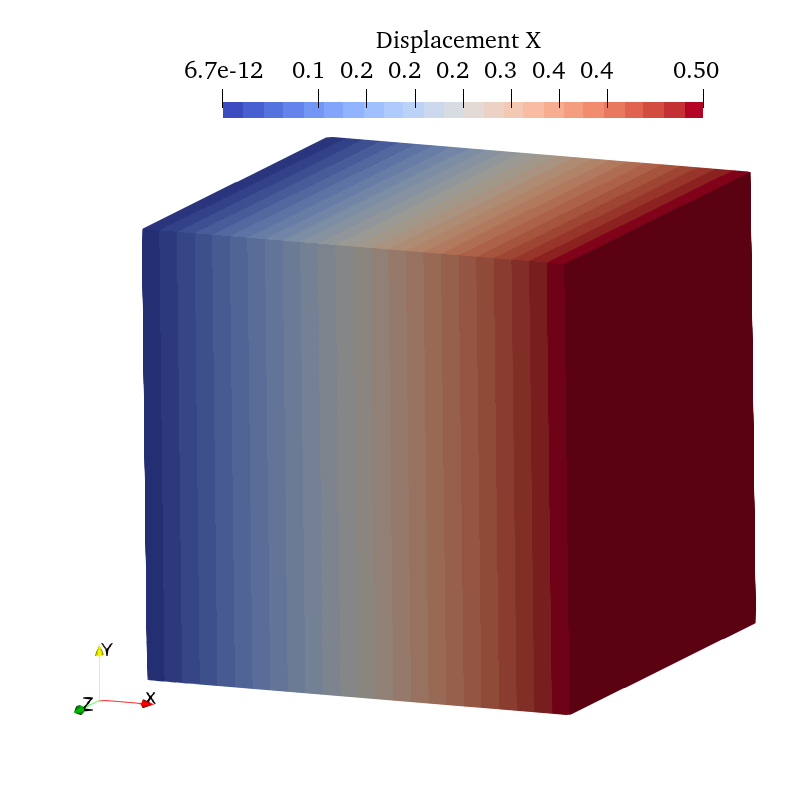
\includegraphics[width=0.4\textwidth,trim={1cm 1.5cm 1.5cm 0cm},clip]{non-homogeneous-stretch-dispx.png}} \qquad
    \subfloat[\label{fig:non-homogeneous-stretch-fields-b}]{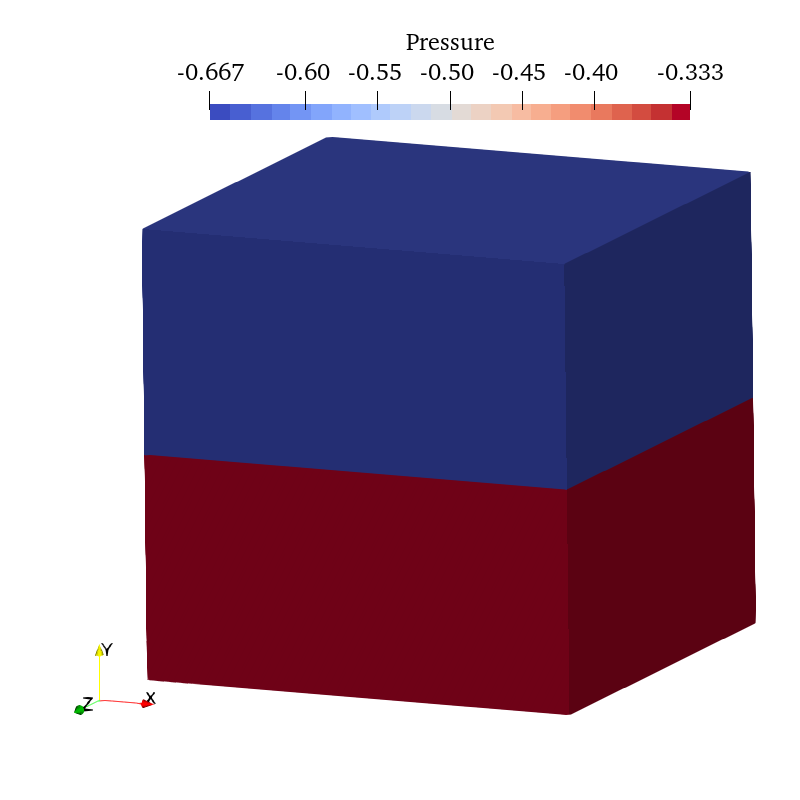
\includegraphics[width=0.4\textwidth,trim={1cm 1.5cm 1.5cm 0cm},clip]{non-homogeneous-stretch-pressure.png}} \\
    \subfloat[\label{fig:non-homogeneous-stretch-fields-c}]
    {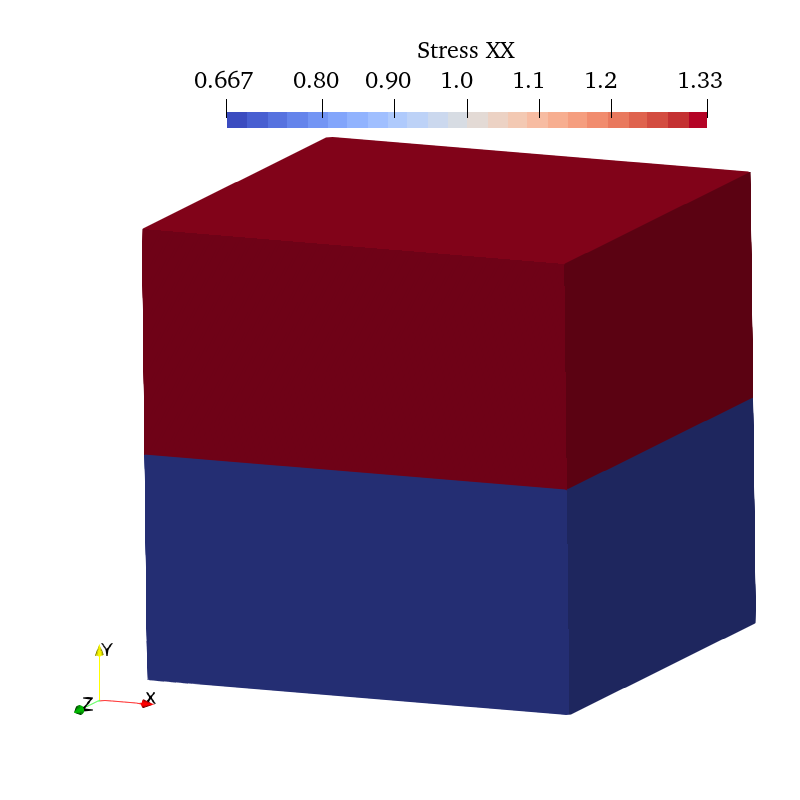
\includegraphics[width=0.4\textwidth,trim={1cm 1.5cm 1.5cm 0cm},clip]{non-homogeneous-stretch-stressxx.png}} \qquad
	\subfloat[\label{fig:non-homogeneous-stretch-fields-d}]
    {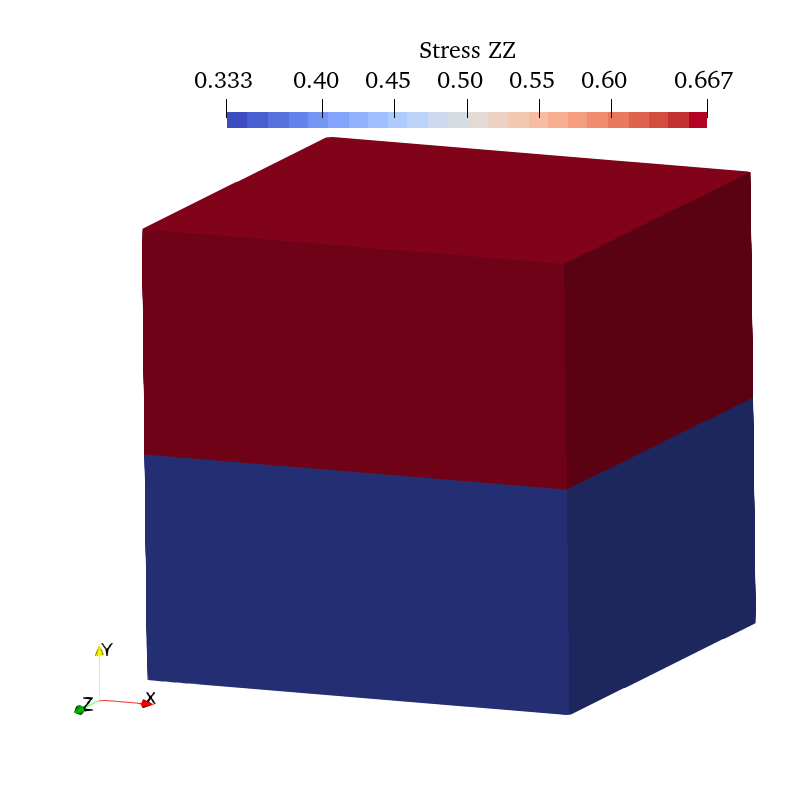
\includegraphics[width=0.4\textwidth,trim={1cm 1.5cm 1.5cm 0cm},clip]{non-homogeneous-stretch-stresszz.png}}
    \caption{Uniform stretch of a non-homogeneous material. (a) $u_x$, (b) $p$, (c) $\sigma_{xx}$ and (d) $\sigma_{zz}$ fields}
    \label{fig:non-homogeneous-stretch-fields}
\end{figure}

\subsection{Cantilever beam subjected to an end shear load \label{subsec:bishop}}

The case of a tridimensional cantilever beam under an end shear-load is considered. Its initial geometry is depicted in Figure \ref{fig:bishop-beam-geometry}, with $L=5$, $a=0.5$, $b=0.5$. The beam is assumed to be fixed at $z=0$ and subjected to a shear-force $F=1$ at $z=L$ pointing downwards in the $y$ direction, while the other faces are traction-free. The material is assumed to have a linear isotropic behaviour with a constant Young modulus $E=1$ whereas different values are used for the poisson coefficient in order to test the formulation for a wide range of compressibility.

\begin{figure}[H]
	\centering
	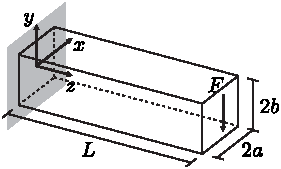
\includegraphics[scale=1.0]{bishop-beam-geometry}
	\caption{Cantilever beam subjected to an end shear load - geometry}
	\label{fig:bishop-beam-geometry}
\end{figure}

The analytical stress state for the problem is given in \cite{bishop2014displacement} and written below:
\begin{equation} \label{eq:bishop-stress}
	\begin{aligned}
		\sigma_{xx} &= \sigma_{xy} = \sigma_{yy} = 0 \text{,}\\
		\sigma_{zz} &= \frac{F}{I} yz \text{,}\\
		\sigma_{xz} &= \frac{F}{I} \frac{2a^2}{\pi^2}\frac{\nu}{1+\nu} \sum_{n=1}^{\infty} \frac{(-1)^n}{n^2} \text{sin}\left(n\pi x/a\right) \frac{\text{sinh}\left( n\pi y/a \right)}{\text{cosh}\left( n\pi b/a \right)} \text{,}\\
		\sigma_{yz} &= \frac{F}{I} \frac{b^2-y^2}{2} + \frac{F}{I}\frac{\nu}{1+\nu} \left[ \frac{3x^2-a^2}{6} - \frac{2a^2}{\pi^2} \sum_{n=1}^{\infty} \frac{(-1)^n}{n^2} \text{cos}\left(n\pi x/a\right) \frac{\text{cosh}\left( n\pi y/a \right)}{\text{cosh}\left( n\pi b/a \right)}  \right]\text{,}\\
	\end{aligned}
\end{equation}

\noindent where $F=\int_{-b}^{b}\int_{-a}^{a}\sigma_{yz}dxdy$ and $I=4ab^3/3$ is the second moment of area about the $x$-axis. The following displacement field is obtained by integrating Equations \eqref{eq:bishop-stress} and enforcing compatibility constrains:
\begin{equation} \label{eq:bishop-displacement}
	\begin{split}
		u_x & = -\frac{F\nu}{EI} xyz \text{,}\\
		u_y & = \frac{F}{EI} \left[ \frac{\nu}{2}\left(x^2-y^2\right)z - \frac{1}{6}z^3 \right] \text{,}\\
		u_z & = \frac{F}{EI} \left[ \frac{1}{2y}\left(\nu x^2+z^2\right)z + \frac{1}{6}\nu y^3 +(1+\nu) \left(b^2 y -\frac{1}{3}y^3\right) -\frac{1}{3}a^2 \nu y \right. \\
		&\qquad\quad \left.-\frac{4a^3\nu}{\pi^3} \sum_{n=1}^{\infty} \frac{(-1)^n}{n^3} \text{cos}\left(n\pi x/a\right) \frac{\text{sinh}\left( n\pi y/a \right)}{\text{cosh}\left( n\pi b/a \right)} \right] \text{.}
	\end{split}
\end{equation}

For the analyses that follow, we kept the number of terms in the series above bounded to $n=5$. The exact solution evaluated on the boundaries of the beam is used to define the boundary conditions for the numerical analysis. At $z=0$, the exact normal and tangential displacements computed according to Eq. \eqref{eq:bishop-displacement} are prescribed, whereas surface tractions in accordance to Eq. \eqref{eq:bishop-stress} are applied on the other five faces.

Two types of partitions are used, with tetrahedra and hexahedra elements. For both cases, the average element size is computed as $h_e=1/2^{n-1}$, where $n=\{1,2,3,4,5\}$. The coarsest ($h_e=1$) and finest ($h_e=0.0625$) meshes for each partition are shown in Figure \ref{fig:bishop-meshes}. The first analysis is carried out keeping $\nu=0.3$ as in the reference \cite{bishop2014displacement}, and a convergence test is performed for the displacement, pressure, stress and mass conservation $L^2$-norm errors.

\begin{figure}[H]
	\centering
	\subfloat[Hexahedral meshes. Coarsest (left) and finest (right)]{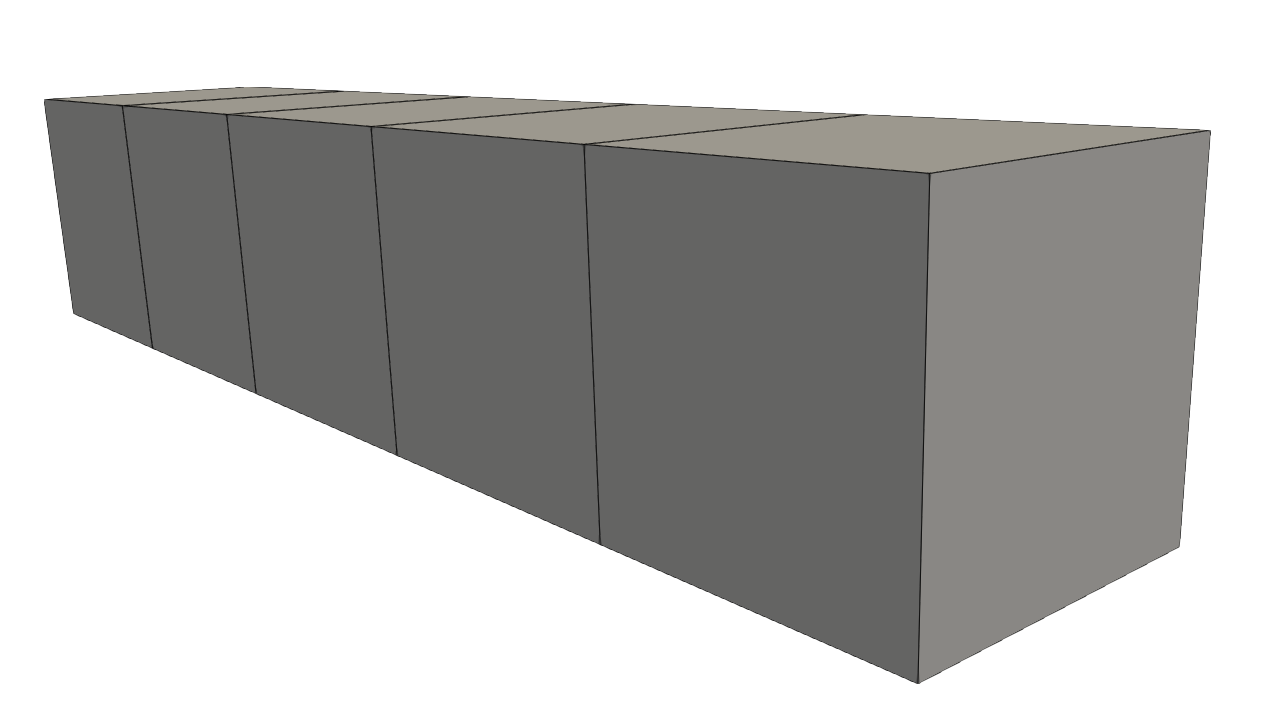
\includegraphics[width=0.48\textwidth]{bishop-mesh-hex-a.png}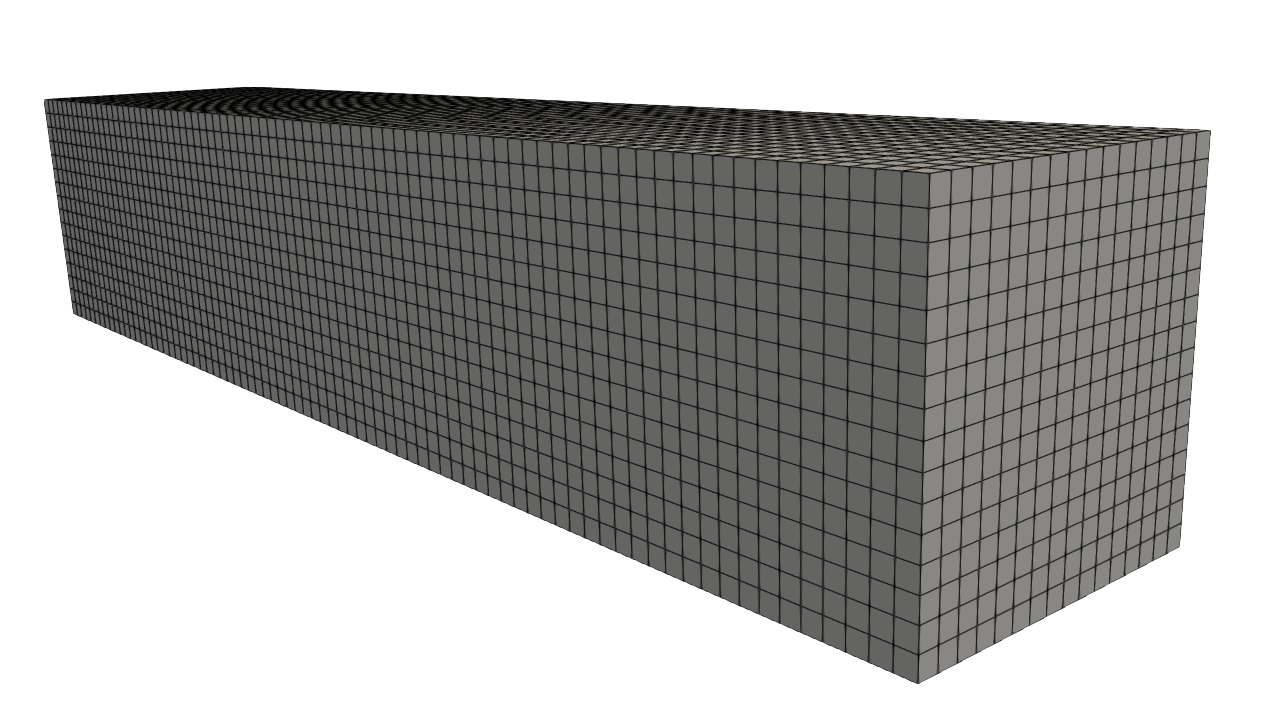
\includegraphics[width=0.48\textwidth]{bishop-mesh-hex-b.png}} \\
	\subfloat[Tetrahedral meshes. Coarsest (left) and finest (right)]{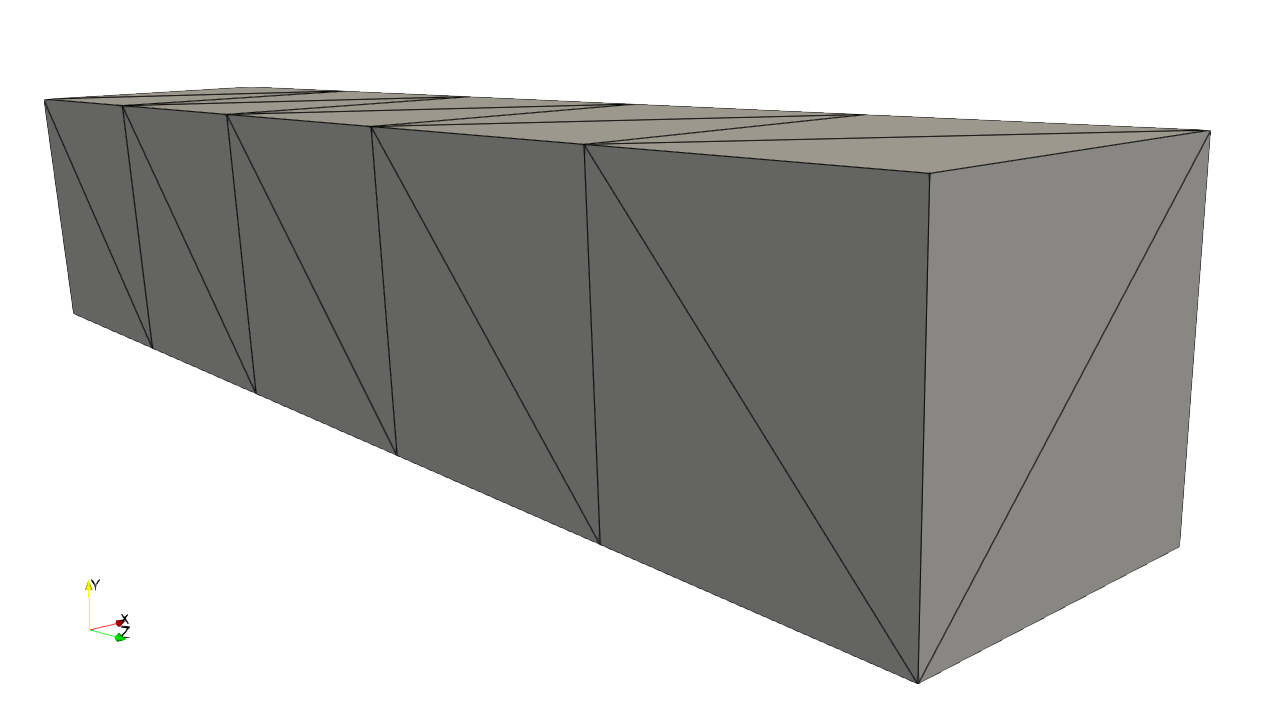
\includegraphics[width=0.48\textwidth]{bishop-mesh-tet-a.png}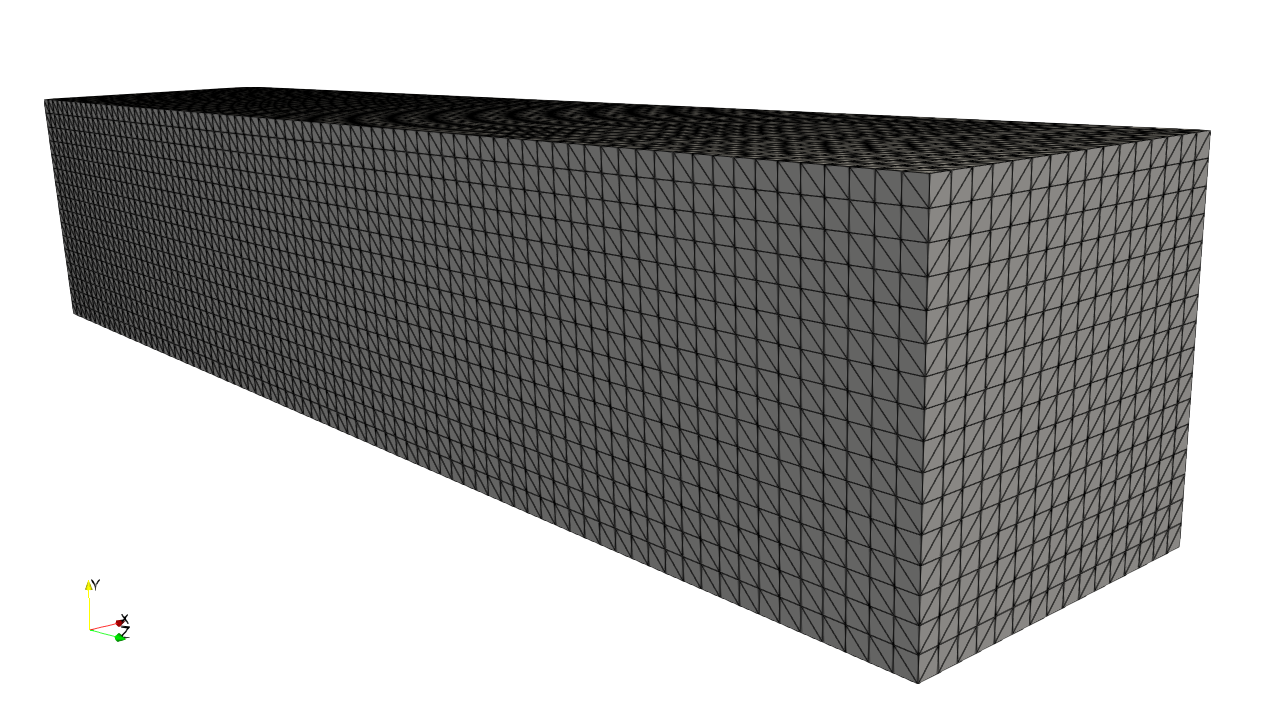
\includegraphics[width=0.48\textwidth]{bishop-mesh-tet-b.png}}
	\caption{Cantilever beam subjected to an end shear load. Meshes used for the convergence test}
	\label{fig:bishop-meshes}
\end{figure}

The results in Figure \ref{fig:bishop-convergence-nu-03} are very similar using both partitions, where optimal convergence rates of order $k+1$ for the displacement and $k$ for the remaining variables are achieved. Figure \ref{fig:bishop-snapshot} plots the displacement, pressure, stress magnitude and von mises stress distributions obtained with the finest hexahedral mesh using $k=3$ over the deformed configuration beam. The results qualitatively agress with the reference solution \cite{bishop2014displacement}.

\begin{figure}[H]
    \centering
    \subfloat[\label{fig:bishop-convergence-nu-03-a}Displacement]{\includetikz{bishop-hex-disp-03}\includetikz{bishop-tet-disp-03}} \\
	\subfloat[\label{fig:bishop-convergence-nu-03-b}Pressure]{\includetikz{bishop-hex-pres-03}\includetikz{bishop-tet-pres-03}} \\
	\subfloat[\label{fig:bishop-convergence-nu-03-c}Stress]{\includetikz{bishop-hex-stress-03}\includetikz{bishop-tet-stress-03}} \\
	\subfloat[\label{fig:bishop-convergence-nu-03-d}Volumetric strain]{\includetikz{bishop-hex-div-03}\includetikz{bishop-tet-div-03}}
    \caption{Cantilever beam subjected to an end shear load. Convergence analysis for the compressible case ($\nu=0.3$) with hexahedral (at left) and tetrahedral (at right) elements using the DHM-H(div) formulation}
    \label{fig:bishop-convergence-nu-03}
\end{figure}

\begin{figure}[H]
    \centering
    \subfloat[\label{fig:bishop-snapshot-a}Displacement]{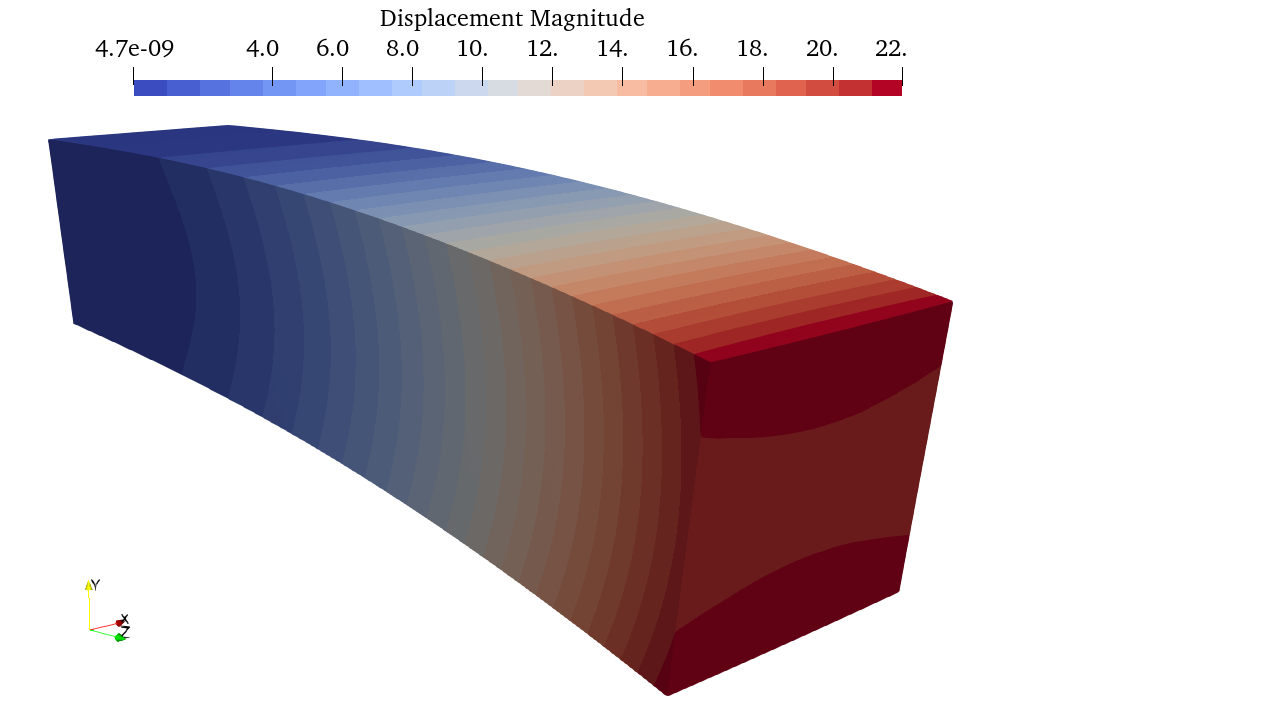
\includegraphics[width=0.47\textwidth,trim={0 0 10cm 0}, clip]{bishop-disp.png}} \hfill
    \subfloat[\label{fig:bishop-snapshot-b}Pressure]{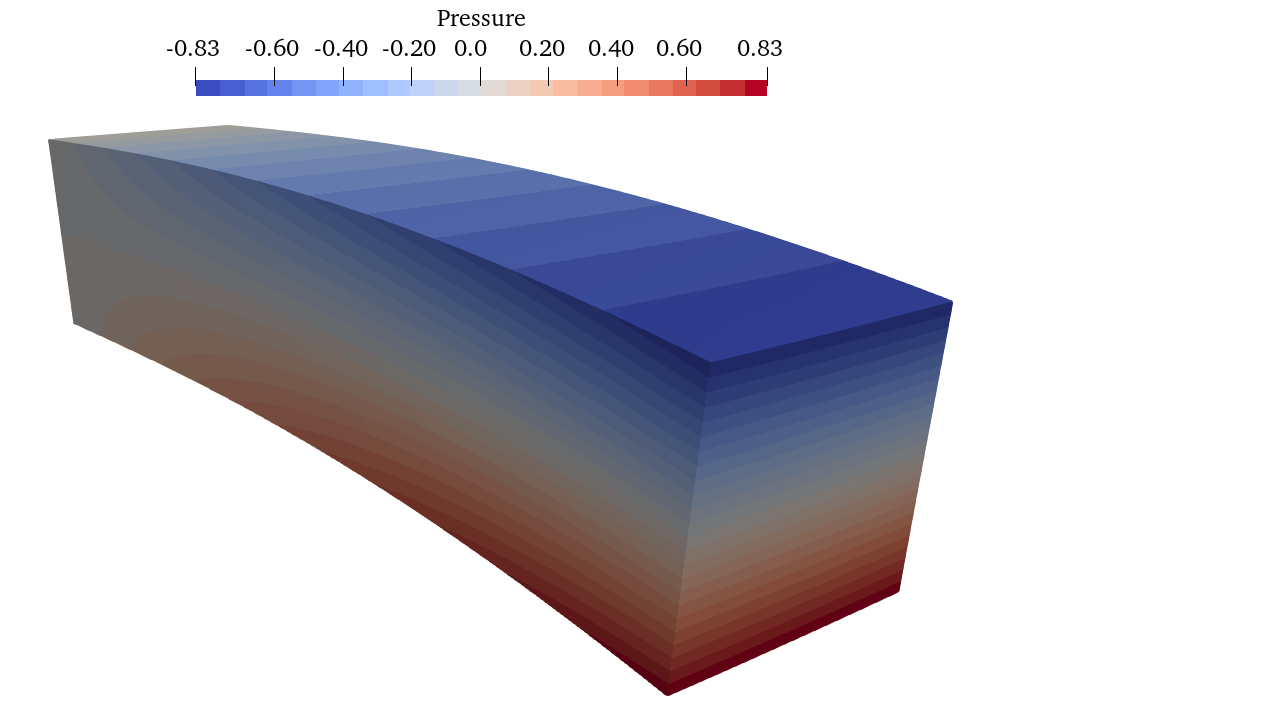
\includegraphics[width=0.47\textwidth,trim={0 0 10cm 0}, clip]{bishop-pressure.png}} \\
    \subfloat[\label{fig:bishop-snapshot-c}Stress magnitude]{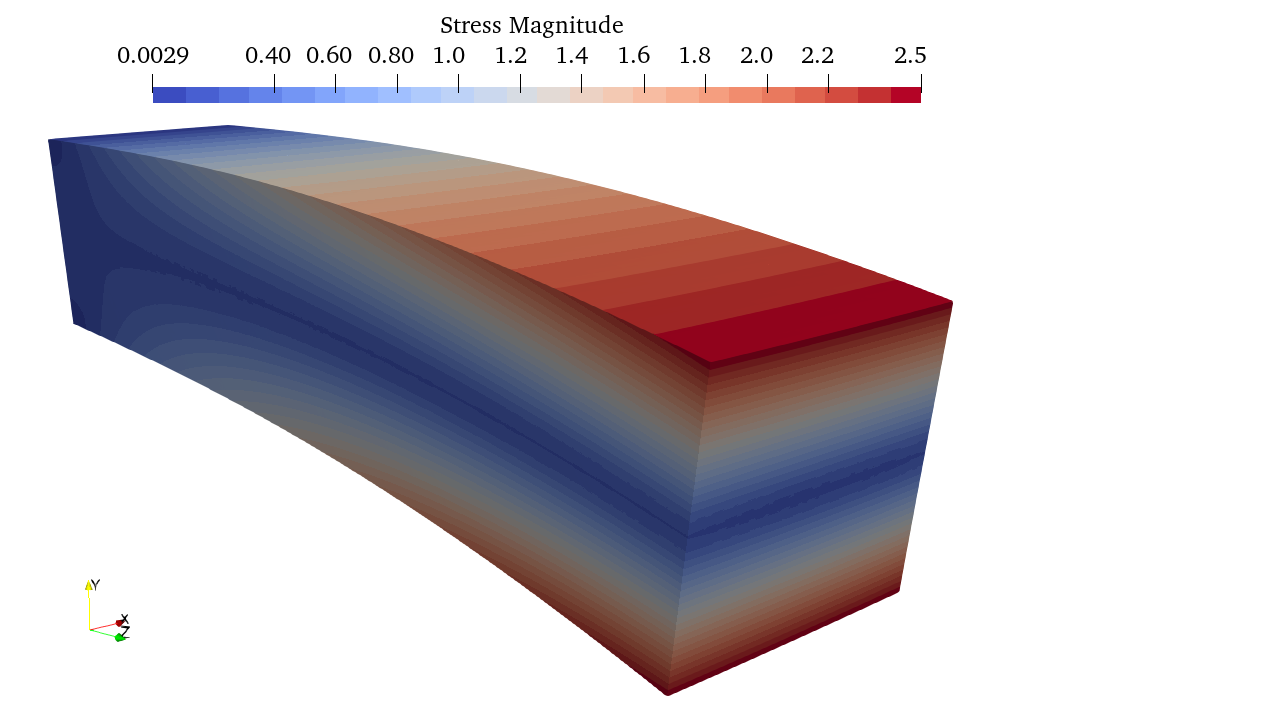
\includegraphics[width=0.47\textwidth,trim={0 0 10cm 0}, clip]{bishop-stress.png}} \hfill
    \subfloat[\label{fig:bishop-snapshot-d}Von Mises stress]{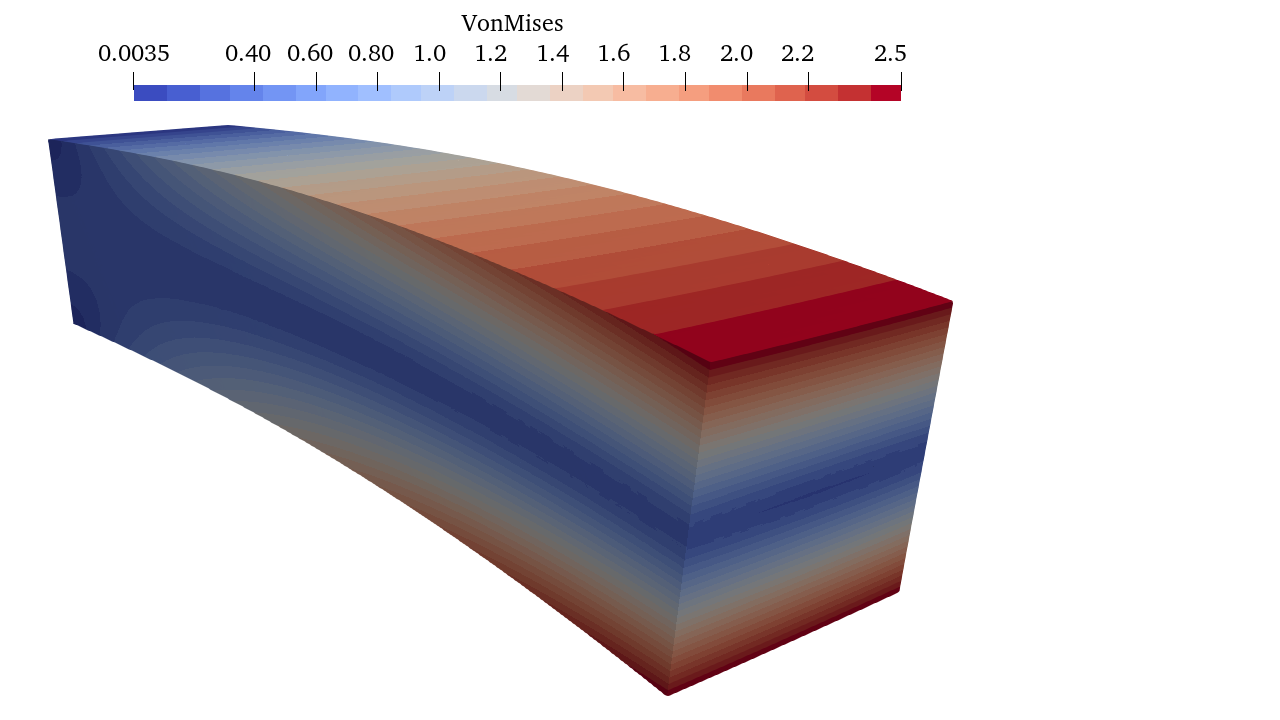
\includegraphics[width=0.47\textwidth,trim={0 0 10cm 0}, clip]{bishop-vonmises.png}}
    \caption{Cantilever beam subjected to an end shear load. Snapshots for $\nu=0.3$}
    \label{fig:bishop-snapshot}
\end{figure}

In order to assess the proposed methodology in different compressibility regimes, Tables \ref{tab:bishop-convergence-049}-\ref{tab:bishop-convergence-050} show the convergence results for $\nu=0.49$, $\nu=0.4999$ and $\nu=0.5$ as well. Optimal convergence rates are achieved independently of the poisson coefficient. This is a nice feature as many formulations present locking under quasi and full incompressibility. Also, for the incompressible case ($\nu=0.5$), a divergence free displacement field is obtained even for the coarsest mesh, with the error bounded to the machine precision.

\begin{table}[H]
    \centering
    \caption{Cantilever beam subjected to an end shear load. Convergence analysis with $\nu=0.49$ for $\bm{u}$, $p$, $\bm{\sigma}$ and $\nabla \cdot \bm{u}$ using hexahedral (at left) and tetrahedral (at right) meshes}
    \vspace{5pt}
	\resizebox{\textwidth}{!}{
    \begin{tabular}{c c c c c | c c c c}
        \toprule
        \multicolumn{5}{c}{\textbf{Hexahedral elements}} & \multicolumn{4}{c}{\textbf{Tetrahedral elements}} \\
        \cmidrule(r){1-5} \cmidrule(l){6-9}
        $h_e$ & $\|\mathbf{u} - \mathbf{u}_h\|$ & $\|p - p_h\|$ & $\|\boldsymbol{\sigma} - \boldsymbol{\sigma}_h\|$ & $\|\nabla \cdot (\mathbf{u} - \mathbf{u}_h)\|$ & $\|\mathbf{u} - \mathbf{u}_h\|$ & $\|p - p_h\|$ & $\|\boldsymbol{\sigma} - \boldsymbol{\sigma}_h\|$ & $\|\nabla \cdot (\mathbf{u} - \mathbf{u}_h)\|$ \\
        \midrule
        \multicolumn{9}{l}{$k = 1$} \\
        1       & $3.28E+00$ & $4.86E-01$ & $1.11E+00$ & $2.34E-13$ & -- & -- & -- & -- \\
        0.5     & $8.07E-01$ & $2.43E-01$ & $5.57E-01$ & $3.57E-13$ & -- & -- & -- & -- \\
        0.25    & $2.02E-01$ & $1.21E-01$ & $2.78E-01$ & $4.65E-13$ & -- & -- & -- & -- \\
        0.125   & $5.04E-02$ & $6.07E-02$ & $1.39E-01$ & $7.05E-13$ & -- & -- & -- & -- \\
        0.06125 & $1.26E-02$ & $3.04E-02$ & $6.96E-02$ & $8.03E-13$ & -- & -- & -- & -- \\
        Rate & $2.00$ & $1.00$ & $1.00$ & --- & $2.00$ & $1.00$ & --- & $2.00$ \\
        \midrule
        \multicolumn{9}{l}{$k = 2$} \\
        1       & $1.23E-01$ & $3.58E-02$ & $1.08E-01$ & $4.58E-12$ & -- & -- & -- & -- \\
        0.5     & $7.61E-03$ & $9.32E-03$ & $2.82E-02$ & $1.01E-11$ & -- & -- & -- & -- \\
        0.25    & $5.35E-04$ & $2.37E-03$ & $7.28E-03$ & $1.95E-11$ & -- & -- & -- & -- \\
        0.125   & $4.84E-05$ & $5.96E-04$ & $1.87E-03$ & $3.89E-11$ & -- & -- & -- & -- \\
        0.06125 & $4.99E-06$ & $1.49E-04$ & $4.69E-04$ & $7.94E-11$ & -- & -- & -- & -- \\
        Rate & $3.00$ & $2.00$ & $2.00$ & --- & $3.00$ & $2.00$ & --- & $3.00$ \\
        \midrule
        \multicolumn{9}{l}{$k = 3$} \\
        1       & $2.09E-03$ & $1.84E-03$ & $7.55E-03$ & $2.17E-12$ & -- & -- & -- & -- \\
        0.5     & $1.38E-04$ & $2.79E-04$ & $1.72E-03$ & $4.58E-12$ & -- & -- & -- & -- \\
        0.25    & $8.36E-06$ & $5.81E-05$ & $2.23E-04$ & $7.97E-12$ & -- & -- & -- & -- \\
        0.125   & $5.40E-07$ & $7.29E-06$ & $2.81E-05$ & $1.69E-11$ & -- & -- & -- & -- \\
        0.06125 & $3.40E-08$ & $9.04E-07$ & $3.49E-06$ & $3.50E-11$ & -- & -- & -- & -- \\
		Rate & $4.00$ & $3.00$ & $3.00$ & --- & $4.00$ & $3.00$ & --- & $3.00$ \\
        \bottomrule
    \end{tabular}}
	\label{tab:bishop-convergence-049}
\end{table}

\begin{table}[H]
    \centering
    \caption{Cantilever beam subjected to an end shear load. Convergence analysis with $\nu=0.4999$ for $\bm{u}$, $p$, $\bm{\sigma}$ and $\nabla \cdot \bm{u}$ using hexahedral (at left) and tetrahedral (at right) meshes}
    \vspace{5pt}
	\resizebox{\textwidth}{!}{
    \begin{tabular}{c c c c c | c c c c}
        \toprule
        \multicolumn{5}{c}{\textbf{Hexahedral elements}} & \multicolumn{4}{c}{\textbf{Tetrahedral elements}} \\
        \cmidrule(r){1-5} \cmidrule(l){6-9}
        $h_e$ & $\|\mathbf{u} - \mathbf{u}_h\|$ & $\|p - p_h\|$ & $\|\boldsymbol{\sigma} - \boldsymbol{\sigma}_h\|$ & $\|\nabla \cdot (\mathbf{u} - \mathbf{u}_h)\|$ & $\|\mathbf{u} - \mathbf{u}_h\|$ & $\|p - p_h\|$ & $\|\boldsymbol{\sigma} - \boldsymbol{\sigma}_h\|$ & $\|\nabla \cdot (\mathbf{u} - \mathbf{u}_h)\|$ \\
        \midrule
        \multicolumn{9}{l}{$k = 1$} \\
        1       & $3.28E+00$ & $4.86E-01$ & $1.11E+00$ & $2.34E-13$ & -- & -- & -- & -- \\
        0.5     & $8.07E-01$ & $2.43E-01$ & $5.57E-01$ & $3.57E-13$ & -- & -- & -- & -- \\
        0.25    & $2.02E-01$ & $1.21E-01$ & $2.78E-01$ & $4.65E-13$ & -- & -- & -- & -- \\
        0.125   & $5.04E-02$ & $6.07E-02$ & $1.39E-01$ & $7.05E-13$ & -- & -- & -- & -- \\
        0.06125 & $1.26E-02$ & $3.04E-02$ & $6.96E-02$ & $8.03E-13$ & -- & -- & -- & -- \\
        Rate & $2.00$ & $1.00$ & $1.00$ & --- & $2.00$ & $1.00$ & --- & $2.00$ \\
        \midrule
        \multicolumn{9}{l}{$k = 2$} \\
        1       & $1.23E-01$ & $3.58E-02$ & $1.08E-01$ & $4.58E-12$ & -- & -- & -- & -- \\
        0.5     & $7.61E-03$ & $9.32E-03$ & $2.82E-02$ & $1.01E-11$ & -- & -- & -- & -- \\
        0.25    & $5.35E-04$ & $2.37E-03$ & $7.28E-03$ & $1.95E-11$ & -- & -- & -- & -- \\
        0.125   & $4.84E-05$ & $5.96E-04$ & $1.87E-03$ & $3.89E-11$ & -- & -- & -- & -- \\
        0.06125 & $4.99E-06$ & $1.49E-04$ & $4.69E-04$ & $7.94E-11$ & -- & -- & -- & -- \\
        Rate & $3.00$ & $2.00$ & $2.00$ & --- & $3.00$ & $2.00$ & --- & $3.00$ \\
        \midrule
        \multicolumn{9}{l}{$k = 3$} \\
        1       & $2.09E-03$ & $1.84E-03$ & $7.55E-03$ & $2.17E-12$ & -- & -- & -- & -- \\
        0.5     & $1.38E-04$ & $2.79E-04$ & $1.72E-03$ & $4.58E-12$ & -- & -- & -- & -- \\
        0.25    & $8.36E-06$ & $5.81E-05$ & $2.23E-04$ & $7.97E-12$ & -- & -- & -- & -- \\
        0.125   & $5.40E-07$ & $7.29E-06$ & $2.81E-05$ & $1.69E-11$ & -- & -- & -- & -- \\
        0.06125 & $3.40E-08$ & $9.04E-07$ & $3.49E-06$ & $3.50E-11$ & -- & -- & -- & -- \\
		Rate & $4.00$ & $3.00$ & $3.00$ & --- & $4.00$ & $3.00$ & --- & $3.00$ \\
        \bottomrule
    \end{tabular}}
	\label{tab:bishop-convergence-04999}
\end{table}

\begin{table}[H]
    \centering
    \caption{Cantilever beam subjected to an end shear load. Convergence analysis with $\nu=0.5$ for $\bm{u}$, $p$, $\bm{\sigma}$ and $\nabla \cdot \bm{u}$ using hexahedral (at left) and tetrahedral (at right) meshes}
    \vspace{5pt}
	\resizebox{\textwidth}{!}{
    \begin{tabular}{c c c c c | c c c c}
        \toprule
        \multicolumn{5}{c}{\textbf{Hexahedral elements}} & \multicolumn{4}{c}{\textbf{Tetrahedral elements}} \\
        \cmidrule(r){1-5} \cmidrule(l){6-9}
        $h_e$ & $\|\mathbf{u} - \mathbf{u}_h\|$ & $\|p - p_h\|$ & $\|\boldsymbol{\sigma} - \boldsymbol{\sigma}_h\|$ & $\|\nabla \cdot (\mathbf{u} - \mathbf{u}_h)\|$ & $\|\mathbf{u} - \mathbf{u}_h\|$ & $\|p - p_h\|$ & $\|\boldsymbol{\sigma} - \boldsymbol{\sigma}_h\|$ & $\|\nabla \cdot (\mathbf{u} - \mathbf{u}_h)\|$ \\
        \midrule
        \multicolumn{9}{l}{$k = 1$} \\
        1       & $3.28E+00$ & $4.86E-01$ & $1.11E+00$ & $2.34E-13$ & -- & -- & -- & -- \\
        0.5     & $8.07E-01$ & $2.43E-01$ & $5.57E-01$ & $3.57E-13$ & -- & -- & -- & -- \\
        0.25    & $2.02E-01$ & $1.21E-01$ & $2.78E-01$ & $4.65E-13$ & -- & -- & -- & -- \\
        0.125   & $5.04E-02$ & $6.07E-02$ & $1.39E-01$ & $7.05E-13$ & -- & -- & -- & -- \\
        0.06125 & $1.26E-02$ & $3.04E-02$ & $6.96E-02$ & $8.03E-13$ & -- & -- & -- & -- \\
        Rate & $2.00$ & $1.00$ & $1.00$ & --- & $2.00$ & $1.00$ & --- & $2.00$ \\
        \midrule
        \multicolumn{9}{l}{$k = 2$} \\
        1       & $1.23E-01$ & $3.58E-02$ & $1.08E-01$ & $4.58E-12$ & -- & -- & -- & -- \\
        0.5     & $7.61E-03$ & $9.32E-03$ & $2.82E-02$ & $1.01E-11$ & -- & -- & -- & -- \\
        0.25    & $5.35E-04$ & $2.37E-03$ & $7.28E-03$ & $1.95E-11$ & -- & -- & -- & -- \\
        0.125   & $4.84E-05$ & $5.96E-04$ & $1.87E-03$ & $3.89E-11$ & -- & -- & -- & -- \\
        0.06125 & $4.99E-06$ & $1.49E-04$ & $4.69E-04$ & $7.94E-11$ & -- & -- & -- & -- \\
        Rate & $3.00$ & $2.00$ & $2.00$ & --- & $3.00$ & $2.00$ & --- & $3.00$ \\
        \midrule
        \multicolumn{9}{l}{$k = 3$} \\
        1       & $2.09E-03$ & $1.84E-03$ & $7.55E-03$ & $2.17E-12$ & -- & -- & -- & -- \\
        0.5     & $1.38E-04$ & $2.79E-04$ & $1.72E-03$ & $4.58E-12$ & -- & -- & -- & -- \\
        0.25    & $8.36E-06$ & $5.81E-05$ & $2.23E-04$ & $7.97E-12$ & -- & -- & -- & -- \\
        0.125   & $5.40E-07$ & $7.29E-06$ & $2.81E-05$ & $1.69E-11$ & -- & -- & -- & -- \\
        0.06125 & $3.40E-08$ & $9.04E-07$ & $3.49E-06$ & $3.50E-11$ & -- & -- & -- & -- \\
		Rate & $4.00$ & $3.00$ & $3.00$ & --- & $4.00$ & $3.00$ & --- & $3.00$ \\
        \bottomrule
    \end{tabular}}
	\label{tab:bishop-convergence-050}
\end{table}

To measure the effectiveness of the DHMH(div) method, we compare the error as a function of the number of degrees of freedom in the global system against the Taylor-Hood formulation for $\nu=0.5$. According to Figure \ref{fig:bishop-comparison-TH},  using both partitions. 





\subsection{Cook's membrane \label{subsec:cook}}

The Cook's membrane is a classical benchmark for the study of locking phenomena of incompressible or nearly-incompressible elasticity problems under shear and bending conditions. It consists of a tapered cantilever beam clamped at its left side and subjected to a shear load in the $y$ direction at $x=48$ mm equal to $F=6.25$ N/mm, according to Figure \ref{fig:cooks-geometry}. The material is assumed to have a linear behaviour with a constant Young modulus $E=240.565$ MPa and two different Poisson coefficients were tested according to the references: $\nu=0.4999$ and $\nu=0.4999999$. This problem can be seen in many books and papers, such as in \cite{cook1989concepts,elguedj2008b,cesar1999new}, with different material properties, geometries and boundary conditions. Some works also studied this problem in the regime of large displacements and strains, under elastic and elastoplastic materials \cite{chavan2007locking,elguedj2008b,de1996design}. In this work, we only focus on the linear elastic analysis.

\begin{figure}[H]
    \centering
    \input{cooks-membrane.pdf_tex}
    \caption{Cook's membrane. Geometry.}
    \label{fig:cooks-geometry}
\end{figure}

At first, we perform plane strain analyses using structured meshes with triangular and quadrilateral partitions with uniform refinements, so that the number of elements per edge is given by $N_e=2^n$, with $n={0,1,2,3,4,5}$. Some of the meshes employed are depicted in Figures \ref{fig:cooks-2d-tri-meshes}-\ref{fig:cooks-2d-quad-meshes}.

\begin{figure}[H]
	\centering
	\subfloat[$N_e=1$]{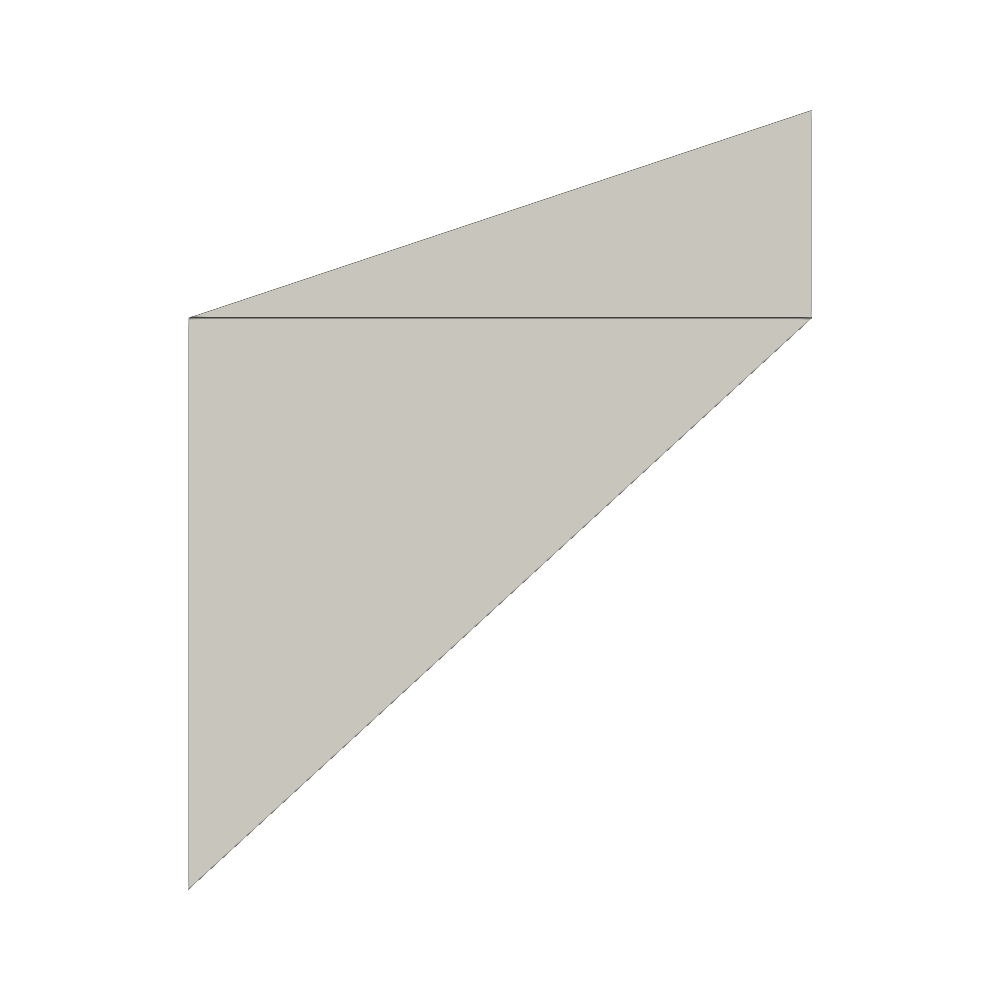
\includegraphics[width=0.25\textwidth, trim={4cm 4cm 4cm 3.5cm}, clip]{cooks-2d-tri-mesh-1.png}}
	\subfloat[$N_e=2$]{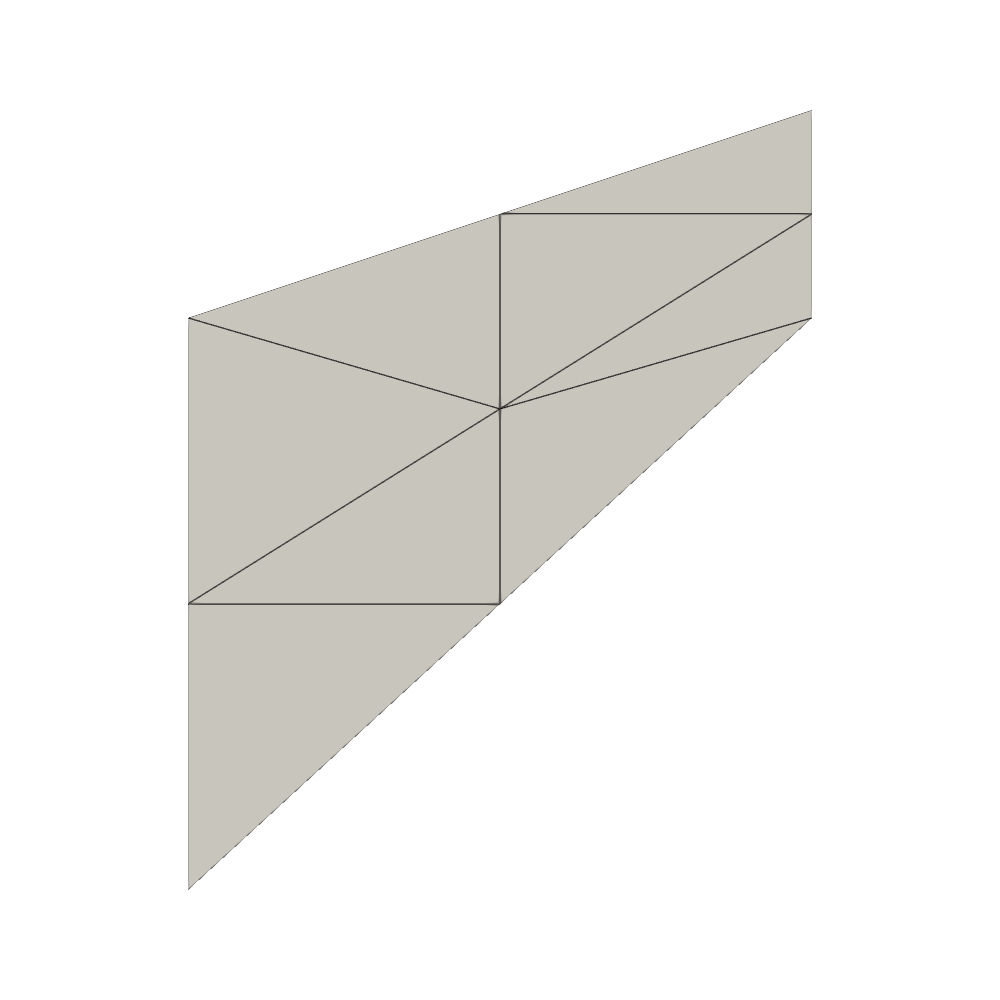
\includegraphics[width=0.25\textwidth, trim={4cm 4cm 4cm 3.5cm}, clip]{cooks-2d-tri-mesh-2.png}}
	\subfloat[$N_e=8$]{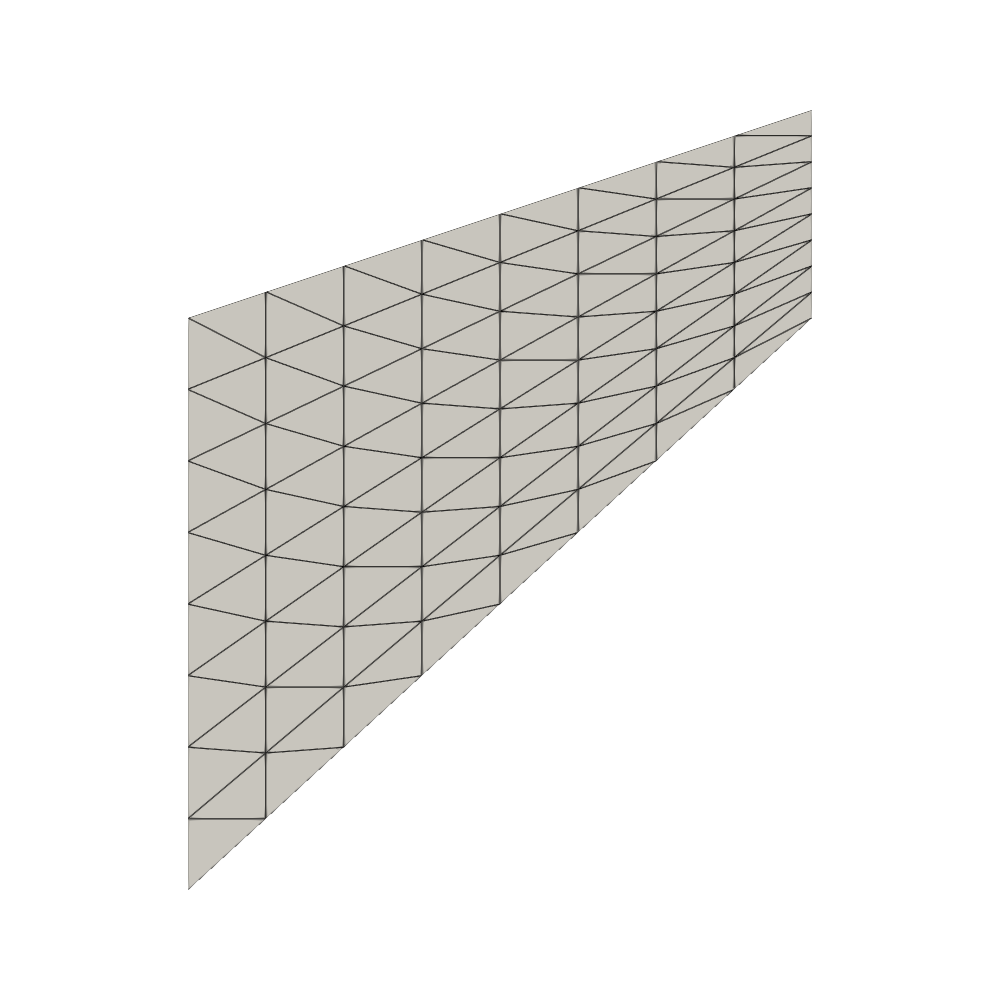
\includegraphics[width=0.25\textwidth, trim={4cm 4cm 4cm 3.5cm}, clip]{cooks-2d-tri-mesh-8.png}}
	\subfloat[$N_e=32$]{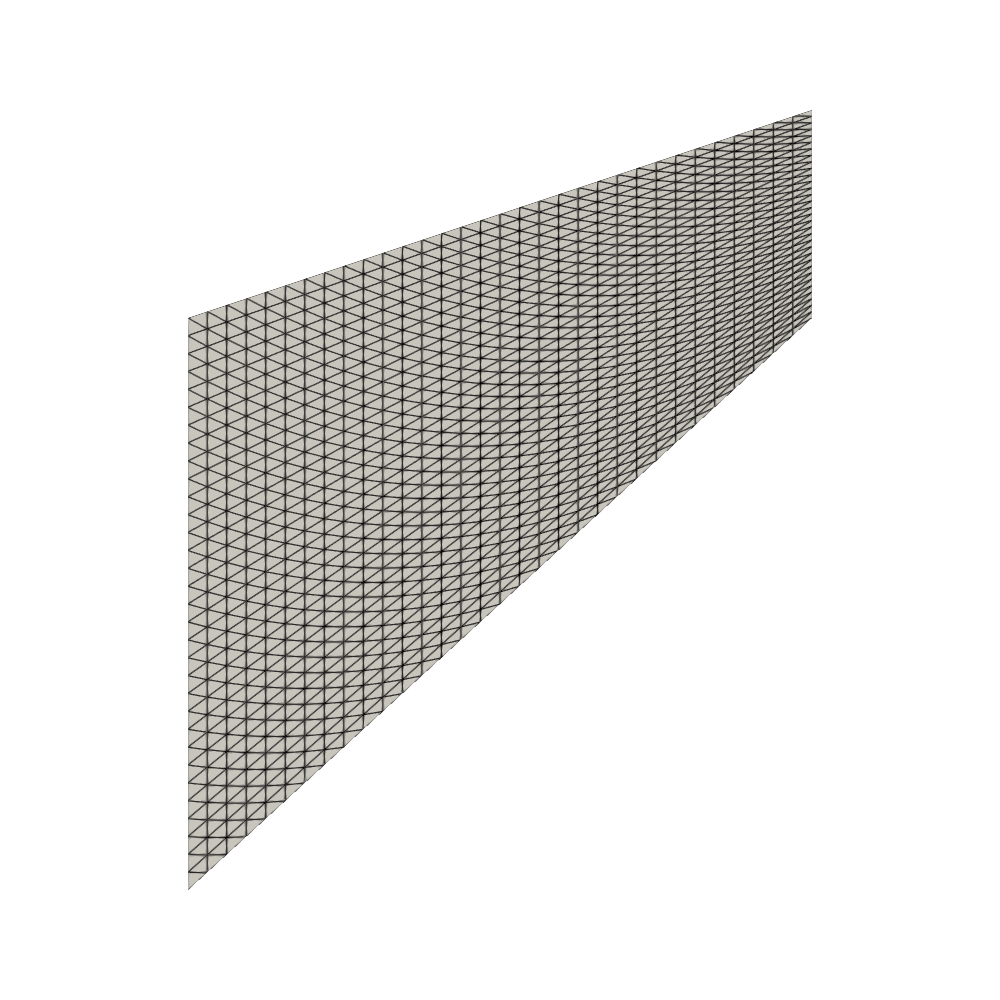
\includegraphics[width=0.25\textwidth, trim={4cm 4cm 4cm 3.5cm}, clip]{cooks-2d-tri-mesh-32.png}}
	\caption{Cook's membrane. Plane strain meshes with triangular partitions.}
	\label{fig:cooks-2d-tri-meshes}
\end{figure}

\begin{figure}[H]
	\centering
	\subfloat[$N_e=1$]{
\includegraphics[width=0.25\textwidth, trim={4cm 4cm 4cm 3.5cm}, clip]{cooks-2d-quad-mesh-1.png}} \hfill
	\subfloat[$N_e=2$]{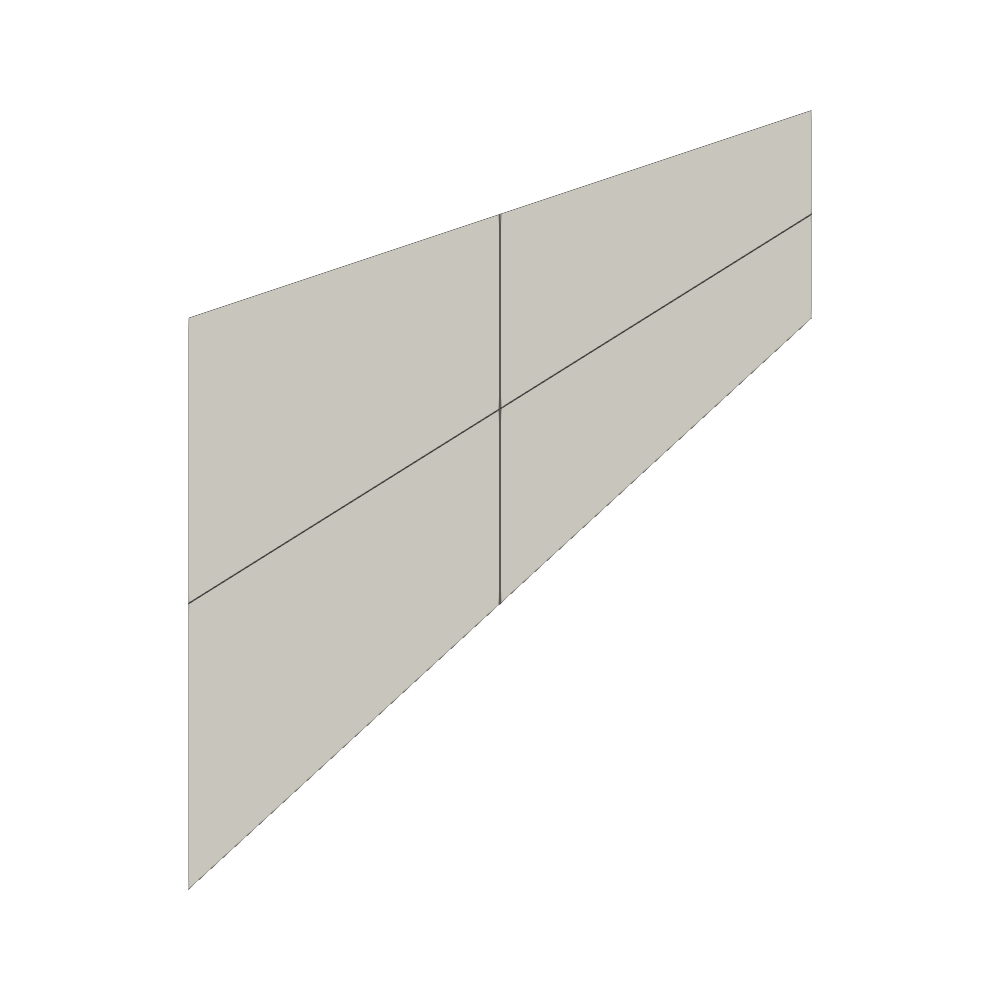
\includegraphics[width=0.25\textwidth, trim={4cm 4cm 4cm 3.5cm}, clip]{cooks-2d-quad-mesh-2.png}} \hfill
	\subfloat[$N_e=8$]{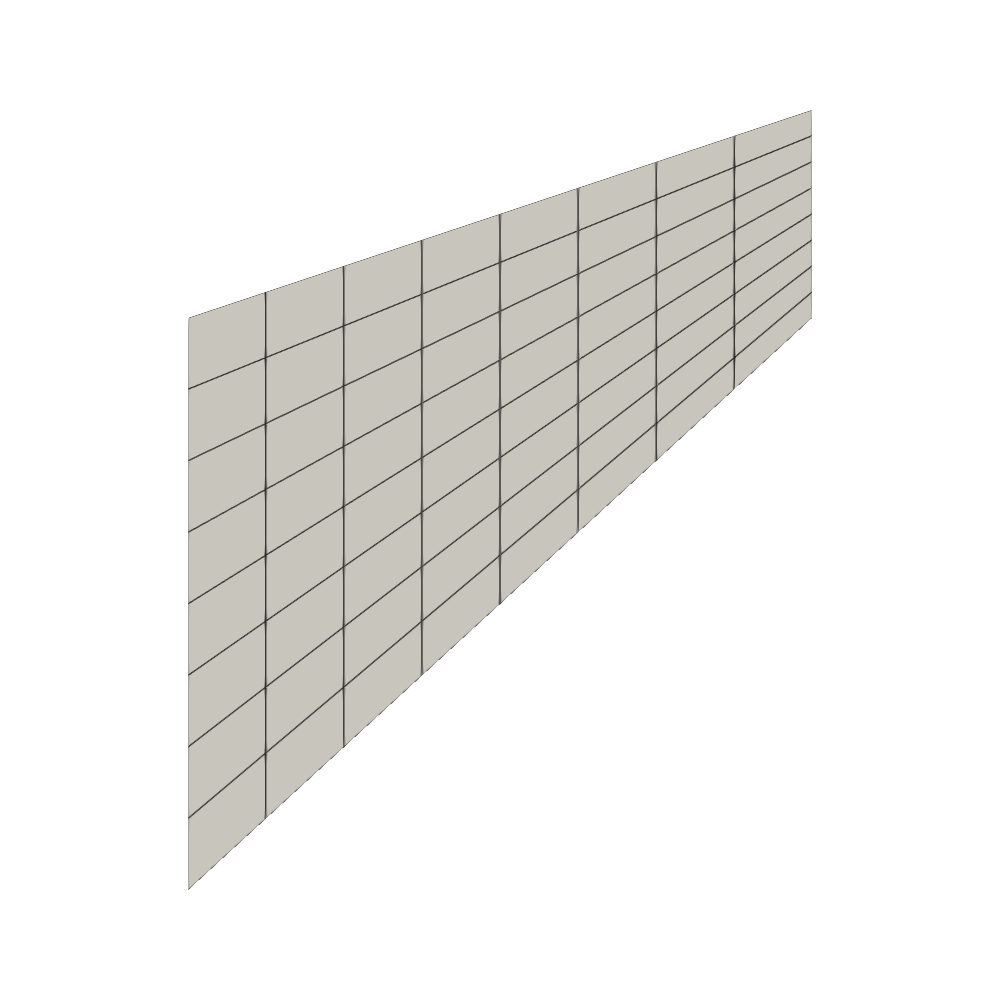
\includegraphics[width=0.25\textwidth, trim={4cm 4cm 4cm 3.5cm}, clip]{cooks-2d-quad-mesh-8.png}} \hfill
	\subfloat[$N_e=32$]{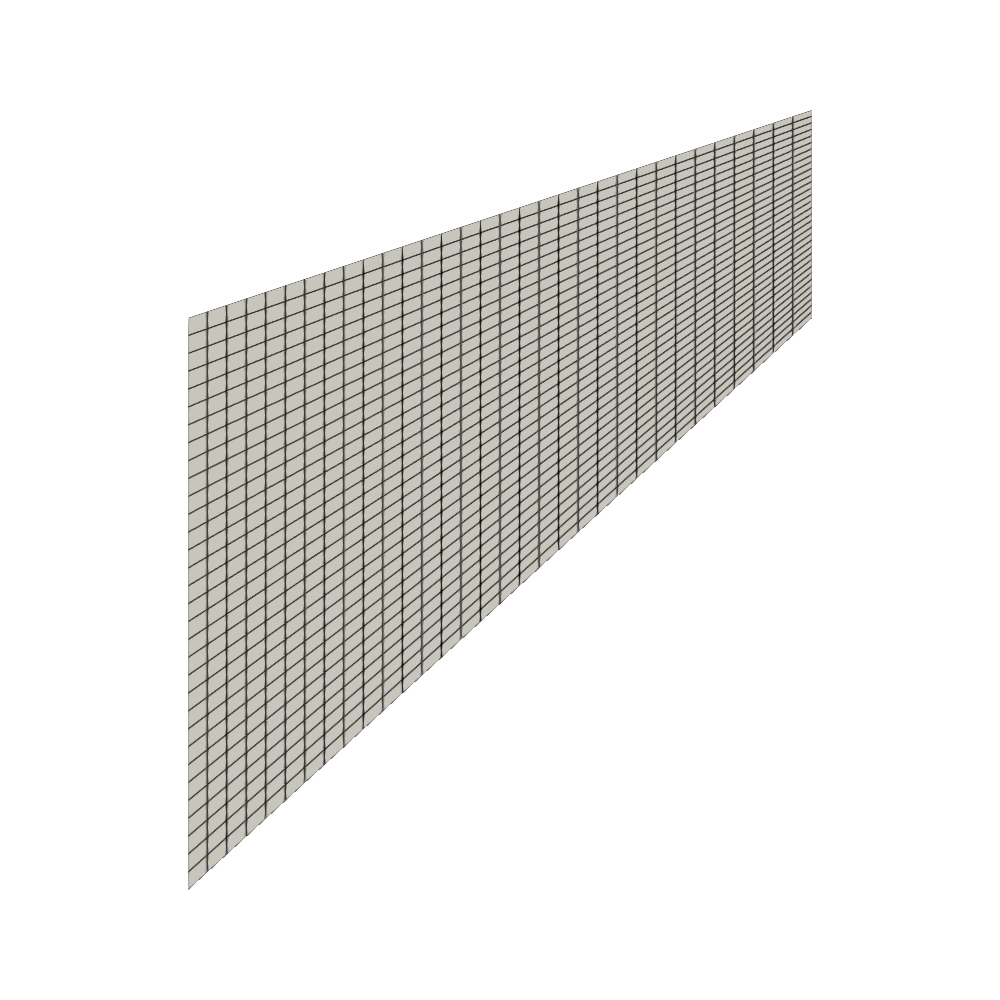
\includegraphics[width=0.25\textwidth, trim={4cm 4cm 4cm 3.5cm}, clip]{cooks-2d-quad-mesh-32.png}}
	\caption{Cook's membrane. Plane strain meshes with quadrilateral partitions.}
	\label{fig:cooks-2d-quad-meshes}
\end{figure}

Figure \ref{fig:cooks-2d-displacement} shows a comparison of the vertical displacement of point A for two values of $\nu$ with some numerical results available in the literature \cite{elguedj2008b,cesar1999new} and results obtained with classical $\mathcal{Q}^1$ and $\mathcal{T}^1$ quadrilateral and triangular elements, respectively, with $H^1$ functions. One notices that our approach leads to a locking-free solution and converges to the reference solutions, while the solutions obtained with classical $H^1$ shape-functions clearly exhibit an excessive bending stiffness leading to a wrong representation of the problem's cinematic.

\begin{figure}[H]
	\centering
	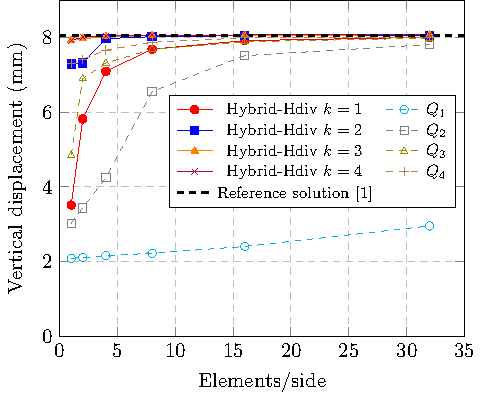
\includegraphics[scale=1.0]{cook-2d-disp-0.4999}
	\caption{Cook's membrane. Vertical displacement of point A.}
	\label{fig:cooks-2d-displacement}
\end{figure}

\subsection{Application problem\label{subsec:module}}

With the objective of testing the method's robustness regarding complex geometries, the proposed methodology is applied to a real-world problem. The geometry of a structural hull is depicted in Figure \ref{fig:module-geometry}, with dimensions $L=1\m$, $r_i=0.345\m$, $r_e=0.390\m$. The hull is subjected to an internal pressure of $p=10.34$ MPa and fixed in the normal direction of all other faces. The material is assumed to have a linear behaviour with a constant Young modulus $E=210000$ MPa and Poisson coefficient $\nu=0.3$. Since the problem is axisymmetric, only one-forth of the domain is modeled, as shown in Figure \ref{fig:module-geometry}. The results obtained with the proposed formulation are compared with the results obtained using the classical Taylor-Hood formulation.

\begin{figure}[h]
    \centering
    \def\svgwidth{450pt} 
    % 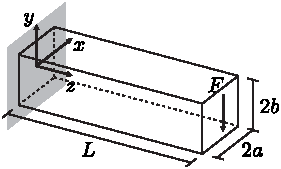
\includegraphics{bishop-beam-geometry.pdf}
    \input{hull-domain.pdf_tex}
    % 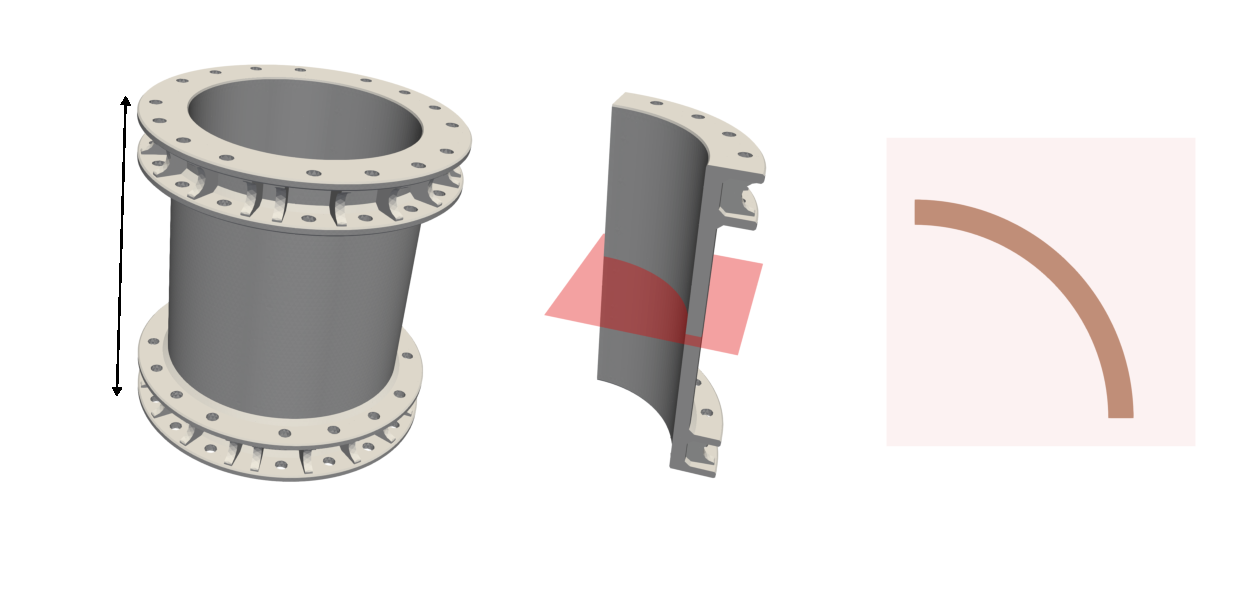
\includegraphics{hull-domain.pdf}
    \caption{Geometry of the structural hull. Only one-forth of the domain is modeled due to axisymmetry of the domain.}
    \label{fig:module-geometry}
\end{figure}

The problem is solved using an unstructured tetrahedral mesh with 68,258 elements, as shown in Figure \ref{fig:module-mesh}. Both the proposed Hybrid-Hdiv and the Taylor-Hood formulations are tested with polynomial degrees $k=2$ and $k=3$, resulting in four different simulations. The results are compared in terms of displacement magnitude, pressure, and Von Mises stresses along a line defined by the points $(259.86, 259.86, 0)$ mm and $(259.86, 259.86, 1000)$ mm. 

The number of degrees of freedom  for the Hybrid-Hdiv formulation is 1,336,260 for $k=2$ and 2,440,900 for $k=3$. For the Taylor-Hood formulation, the number of DOF is 322,447 for $k=2$ and 1,060,639 for $k=3$. The high number of degrees of freedom when using the Hybrid-Hdiv formulation in this problem is due to the use of tetrahedral elements, which increase the number of faces in the mesh. In the Hybrid-Hdiv method, the number of degrees of freedom is significantly influenced by the number of element faces in the mesh.

\begin{figure}[h]
	\centering
	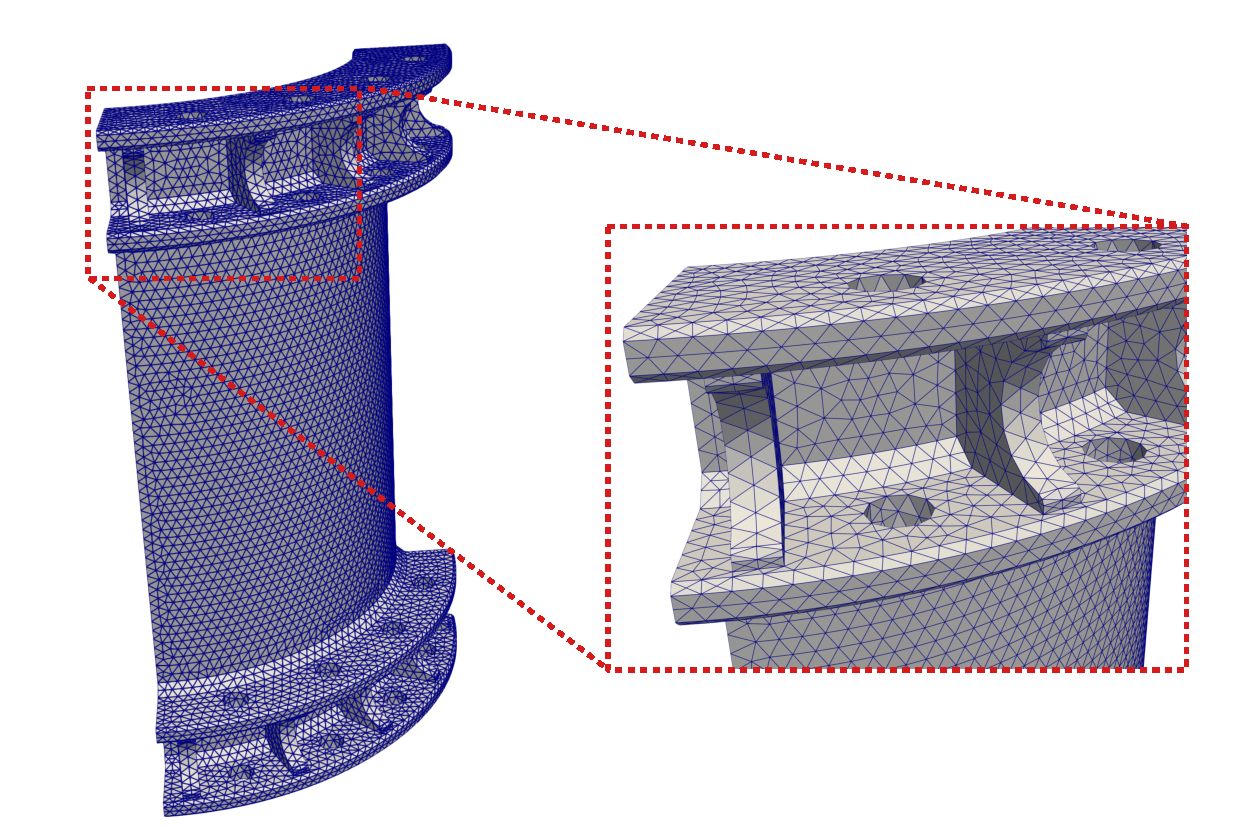
\includegraphics[scale=0.75]{hull-mesh.pdf}
	\caption{Adopted finite element mesh of the hull with zoom in showing the details of the top region of the domain.}
	\label{fig:module-mesh}
\end{figure}

Figure \ref{fig:module-shapes} shows the structural hull in both undeformed and deformed configurations. Subfigure \ref{fig:module-shapes-a} presents the undeformed shape with a color map representing the displacement field, highlighting the regions with higher displacements. Subfigure \ref{fig:module-shapes-b} illustrates the deformed shape (scaled by 2000 for better visualization) with a color map of the Von Mises stress field, indicating the stress distribution throughout the structure.


\begin{figure}[H]
	\centering
	\subfloat[Undeformed shape with displacement field]{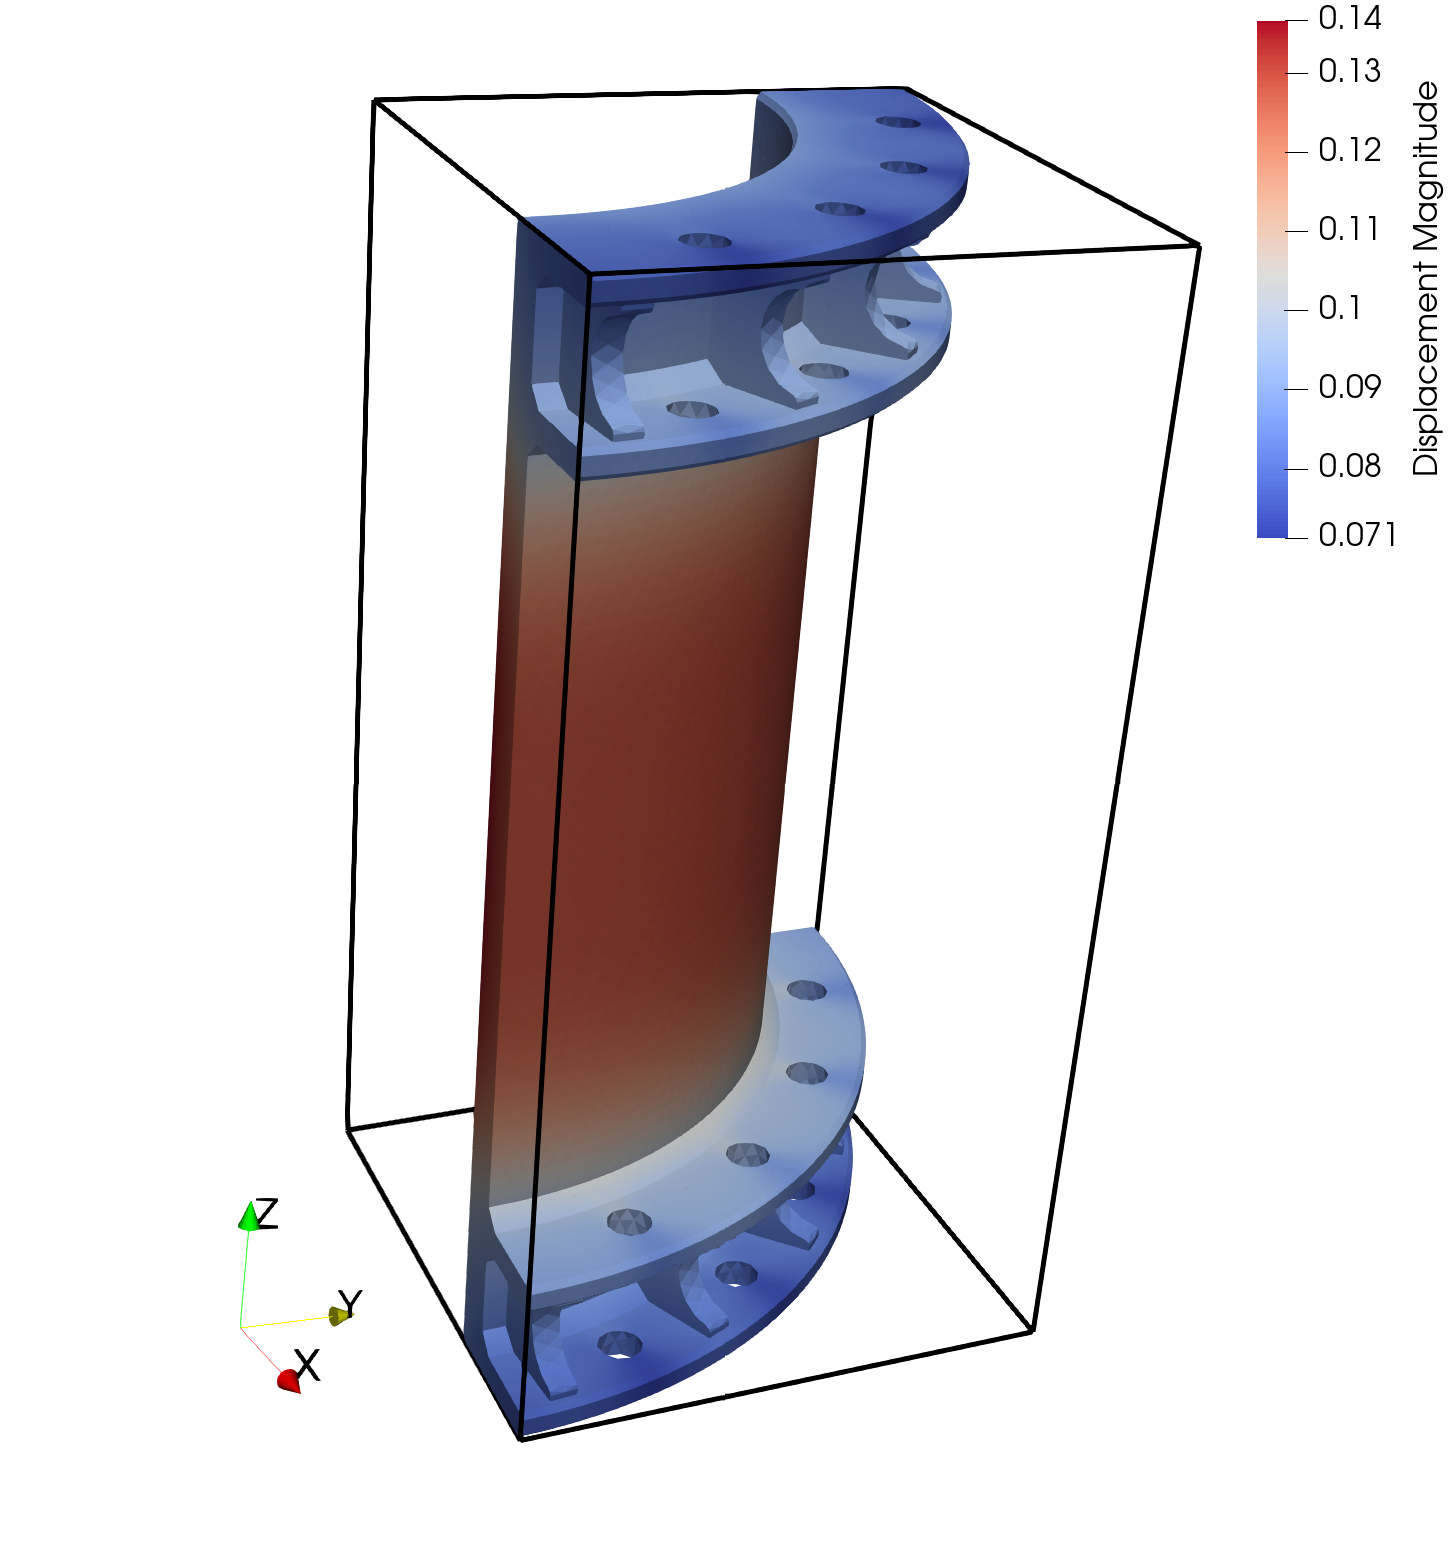
\includegraphics[width=0.45\textwidth]{hull-undeformed.png}\label{fig:module-shapes-a}}
	\hfill
	\subfloat[Deformed shape with Von Mises stress field]{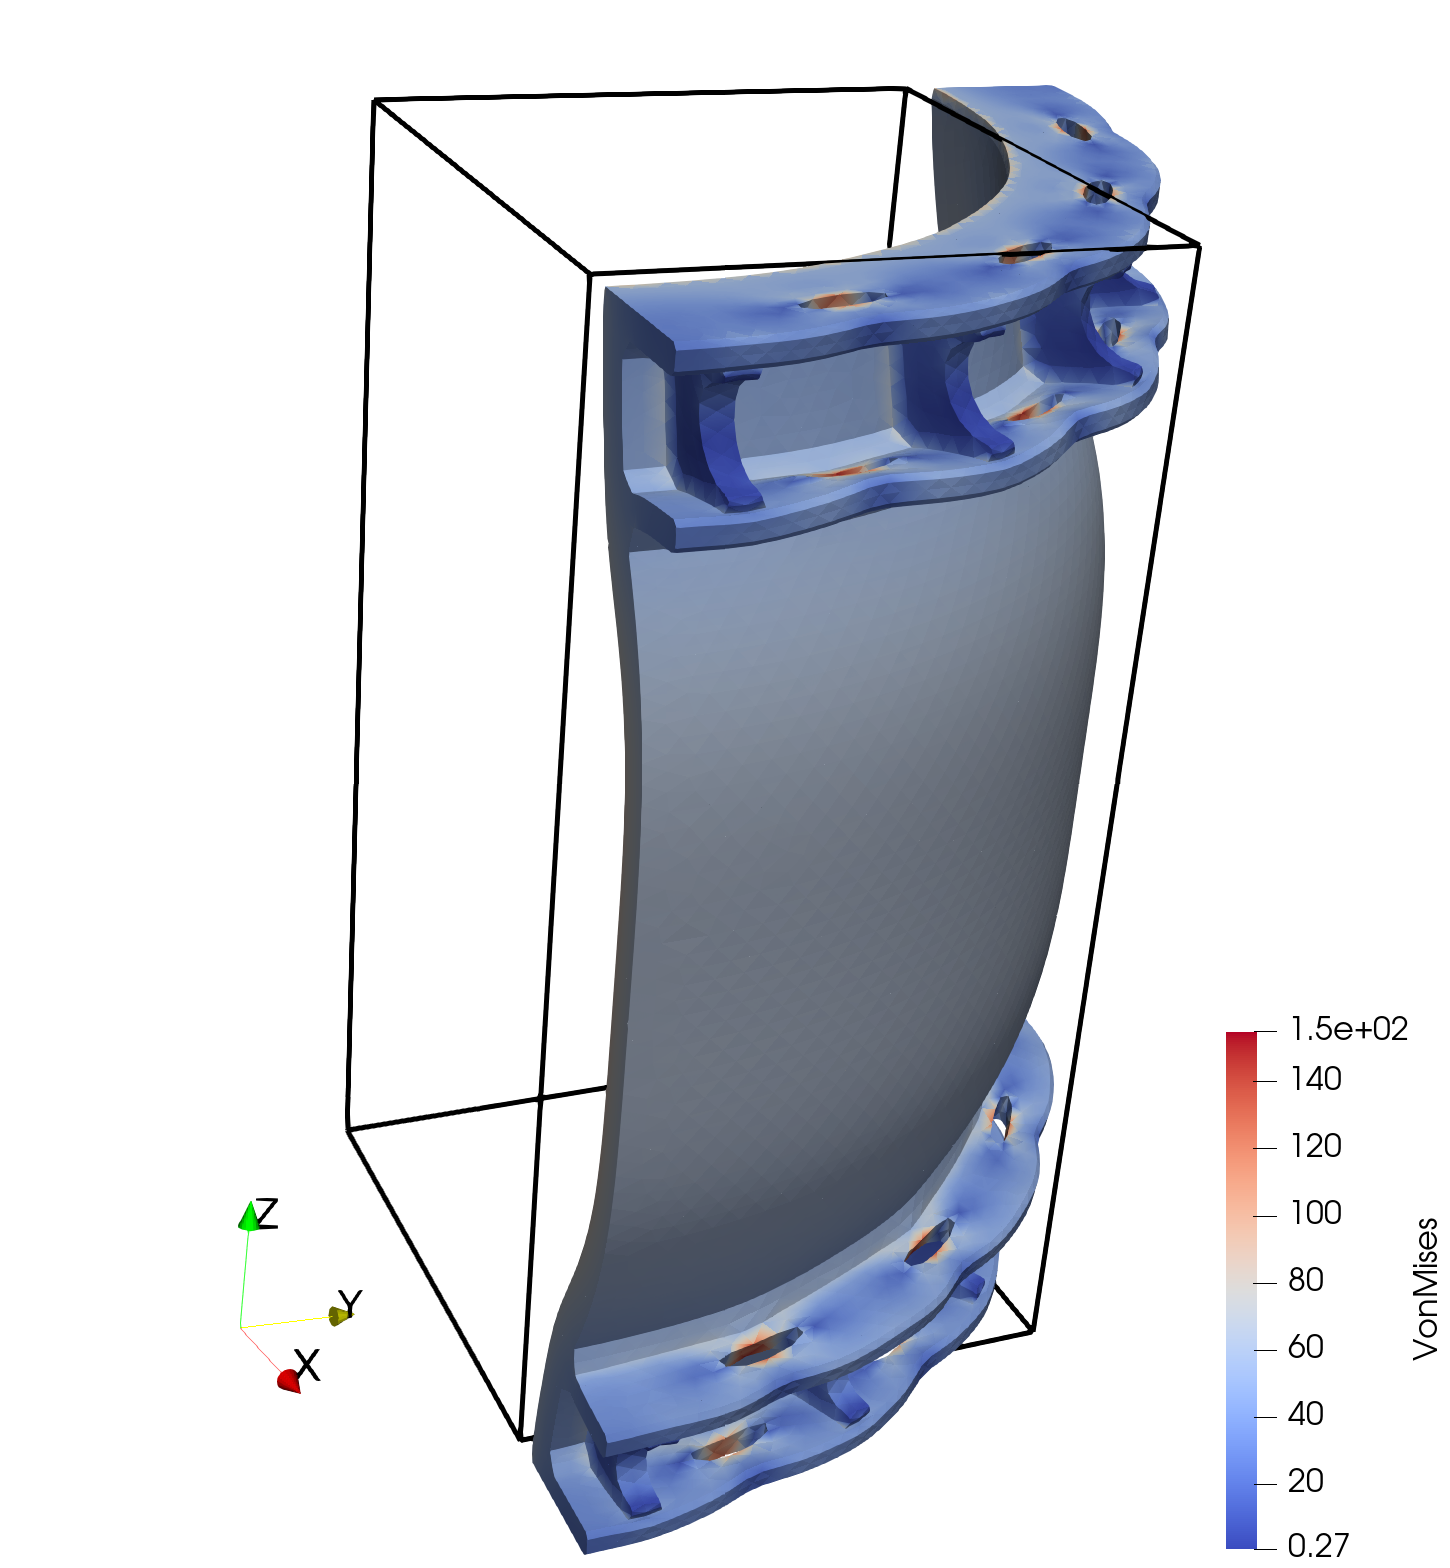
\includegraphics[width=0.45\textwidth]{hull-deformed.png}\label{fig:module-shapes-b}}
	\caption{Structural hull: (a) undeformed shape with displacement field, (b) deformed shape with Von Mises stress field.}
	\label{fig:module-shapes}
\end{figure}

The results for the displacement magnitude, pressure, and Von Mises stresses are shown in Figure \ref{fig:module-results}. The results show that the proposed Hybrid-Hdiv formulation is able to capture the correct stress and displacement distributions for this application example. Smoother solution fields were obtained at the beginning and end of the line for the Hybrid-Hdiv formulation compared to the Taylor-Hood formulation. This is explained by larger amount of degrees of freedom when adopting the Hybrid-Hdiv formulation. 

\begin{figure}[H]
	\centering
	\subfloat[Displacement magnitude]{\includetikz{module_disp}}
	\subfloat[Pressure]{\includetikz{module_pressure}}

	\subfloat[Von Mises Stress]{\includetikz{module_vonmises}}
	\subfloat[Von Mises Stress - Zoom]{\includetikz{module_vonmises_zoom}}
		
	\caption{Comparison of displacement magnitude, pressure, and Von Mises stress distributions along the defined line for the Hybrid-Hdiv and Taylor-Hood formulations with polynomial degrees $k=2$ and $k=3$.\label{fig:module-results}}
	
\end{figure}

\section{Conclusions}

{\giovane A first shot, please give your contributions}
In this work a primal hybrid formulation for tridimensional elasticity problems was developed. The approximation space composed of De Rham compatible $H(\text{div})$ functions for the normal displacements and  $L^2$ functions for the pressure leads to a locally conservative scheme. A second hybridization of the tangential stresses was applied in order to obtain positive semi definite element matrices after condensing internal degrees of freedom. The property of the resulting global system is  symmetric positive-definite matrix when analysing compressible solids and a saddle-point problem with a single mean pressure per element acting as a Lagrange multiplier for incompressible materials.

The formulation was tested for a cantilever beam subjected to an end shear load and the results showed optimal convergence rates of $k+1$ for the displacement and $k$ for the remaining variables independently of the poisson coefficient. The formulation was able to capture the correct stress and displacement distributions for the compressible case and a divergence free displacement field for the incompressible case. The simulation of a real scale structural hull subjected to an internal pressure qualitatively indicates that the proposed method can be applied to real engineering problems.

\bigskip\noindent {\bf Acknowledgments:} Authors  Nat, Gio, Hug, and Phil acknowledge the support from...

%\bibliographystyle{plainnat}
\bibliographystyle{elsarticle-num}
\addcontentsline{toc}{section}{\refname}
\bibliography{%
	references}

\end{document}
